% USEM -- unsymmetric spectral element method (2D elasticity)
% Documentation of the MATLAB code
%
% Build (from this folder):  latexmk -pdf usem-documentation.tex
% or:                        pdflatex, biber, pdflatex, pdflatex
\documentclass[11pt,a4paper,oneside]{report}

\usepackage[T1]{fontenc}
\usepackage[utf8]{inputenc}
\usepackage{lmodern}
\usepackage[english]{babel}
\usepackage{csquotes}
\usepackage{etoolbox}
\usepackage{microtype}
\usepackage[margin=25mm]{geometry}
\usepackage{amsmath,amssymb}
\usepackage{bm}
\usepackage{booktabs}
\usepackage{array}
\usepackage{xltabular}
\usepackage{enumitem}
\usepackage{xcolor}
\usepackage{listings}
\usepackage{url}
\usepackage{tikz}
\usetikzlibrary{arrows.meta,positioning,calc,shapes.geometric,fit,backgrounds}
\usepackage{pgfplots}
\pgfplotsset{compat=1.18}
\usepgfplotslibrary{groupplots}
\usepackage[backend=biber,style=authoryear,maxcitenames=2,uniquelist=false,
            uniquename=false,doi=true,url=false,isbn=false,eprint=false,
            dashed=false]{biblatex}
\addbibresource{../literature/references.bib}
\usepackage[colorlinks=true,linkcolor=blue!50!black,citecolor=green!40!black,
            urlcolor=blue!50!black]{hyperref}
\usepackage[nameinlink,capitalise]{cleveref}

% ---------------------------------------------------------------------------
% Notation and helpers
% ---------------------------------------------------------------------------
% File, function and variable names (underscores allowed, line breaks at /)
\DeclareUrlCommand\code{\urlstyle{tt}}
\renewcommand{\UrlBreaks}{\do\/\do\_\do\.\do\,\do\-\do\=\do\*}
\newcommand{\vect}[1]{\mathbf{#1}}
\newcommand{\matr}[1]{\mathbf{#1}}
\newcommand{\T}{\mathsf{T}}
\newcommand{\dd}{\,\mathrm{d}}
\newcommand{\adj}{\operatorname{adj}}

\lstdefinestyle{matlab}{
  language=Matlab, basicstyle=\ttfamily\small, columns=fullflexible,
  keepspaces=true, commentstyle=\color{green!40!black},
  keywordstyle=\color{blue!60!black}, stringstyle=\color{purple!70!black},
  frame=single, framesep=4pt, rulecolor=\color{black!25},
  backgroundcolor=\color{black!3}, upquote=true, showstringspaces=false}
\lstdefinestyle{shell}{
  basicstyle=\ttfamily\small, columns=fullflexible, keepspaces=true,
  frame=single, framesep=4pt, rulecolor=\color{black!25},
  backgroundcolor=\color{black!3}, upquote=true}
\lstset{style=matlab}

% Table columns
\newcolumntype{L}{>{\raggedright\arraybackslash}X}
\newcolumntype{P}[1]{>{\raggedright\arraybackslash}p{#1}}

% Common TikZ styles
\tikzset{
  node dot/.style={circle, fill=black, inner sep=1.3pt},
  box/.style={draw, rounded corners=2pt, align=center, font=\small,
              inner sep=4pt, fill=white},
  dimarrow/.style={-{Stealth[length=2mm]}, thin},
}

\setlist{itemsep=2pt,topsep=4pt}

% Long identifiers: allow some extra stretch in paragraphs, smaller font in
% tables
\setlength{\emergencystretch}{3em}
\AtBeginEnvironment{xltabular}{\small}
\AtBeginEnvironment{tabularx}{\small}

\title{\textbf{USEM}\\[4pt]
  \large Unsymmetric spectral element method for two-dimensional elasticity\\[2pt]
  \normalsize Documentation of the MATLAB code}
\author{Otto von Guericke University Magdeburg}
\date{\today}

\begin{document}

\maketitle
\tableofcontents

\chapter{Theory: The unsymmetric spectral element method}
\label{ch:theory}

This chapter describes the formulation as it is implemented in
\code{code/subroutines}. The literature is collected in \cref{ch:literature}.

\section{Problem}

The code solves linear plane elasticity on a domain $\Omega$ with thickness 1. In
Voigt notation, the equilibrium equation, Hooke's law and the strains read
\begin{equation}
  \matr L^{\T}\bm\sigma + \vect b = \vect 0,\qquad
  \bm\sigma = \matr C\,\bm\varepsilon,\qquad
  \bm\varepsilon = \matr L\,\vect u =
  \begin{bmatrix}\varepsilon_{xx}\\ \varepsilon_{yy}\\ \gamma_{xy}\end{bmatrix},
  \qquad
  \matr L = \begin{bmatrix}\partial_x & 0\\ 0 & \partial_y\\
                           \partial_y & \partial_x\end{bmatrix},
\end{equation}
where $\vect u$ is the displacement vector, $\bm\sigma$ and $\bm\varepsilon$ are
the stress and strain vectors, $\vect b$ is the body force per unit volume and
$\matr L$ is the differential operator, with prescribed displacements
$\bar{\vect u}$ on the Dirichlet boundary $\Gamma_\mathrm{u}$ and prescribed
tractions $\bar{\vect t}$ on the Neumann boundary $\Gamma_\mathrm{t}$. $\matr C$ is
the $3\times3$ plane stress matrix (\code{HookeMatrix2d}, or condensed from the
three-dimensional Hooke matrix with \code{PlaneStressConstitutiveMatrices}).

\section{Petrov-Galerkin weak form}

The classical (Bubnov-Galerkin) finite or spectral element uses the same
isoparametric shape functions to interpolate the displacements (trial
functions) and to weight the equilibrium equation (test functions). The
unsymmetric element uses two different sets \parencite{Rajendran2010technique},
see \cref{tab:spaces,fig:spaces}.

\begin{table}[htbp]
  \centering
  \caption{Shape functions of the unsymmetric element.}
  \label{tab:spaces}
  \begin{tabular}{@{}lll@{}}
    \toprule
    Role & Shape functions & Property \\
    \midrule
    test (weighting) & parametric, $N_i(\xi,\eta)$ &
      continuous across element edges \\
    trial (displacement) & metric, $M_j(x,y)$ &
      complete polynomials in $x$ and $y$ \\
    \bottomrule
  \end{tabular}
\end{table}

\begin{figure}[htbp]
  \centering
  % Reference element (parametric test functions) and distorted element with
% corotational skew coordinates (metric trial functions)
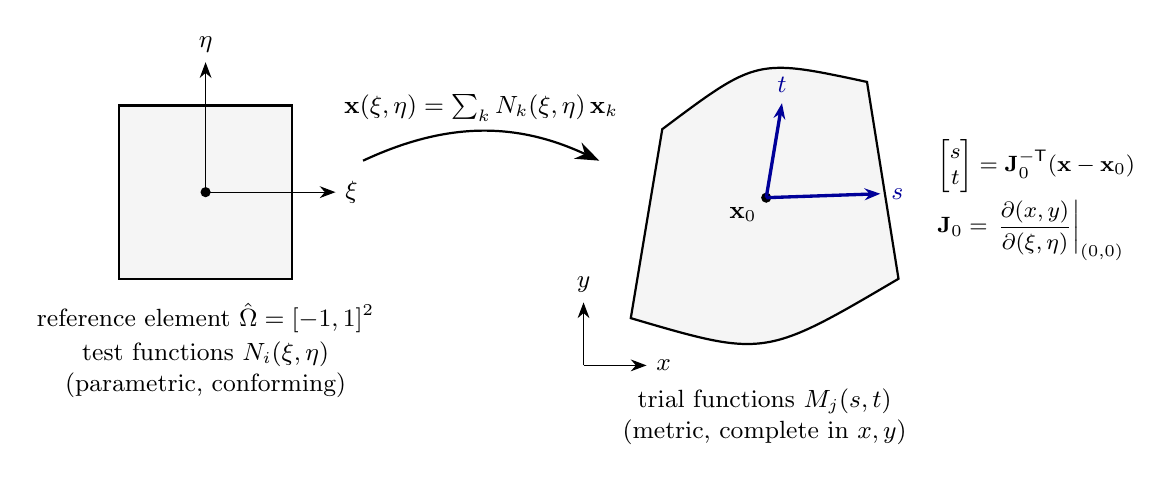
\begin{tikzpicture}[every node/.style={font=\small}]
  % ---- reference element ----
  \begin{scope}[scale=1.1]
    \draw[thick, fill=black!4] (-1,-1) rectangle (1,1);
    \draw[dimarrow] (0,0) -- (1.5,0) node[right] {$\xi$};
    \draw[dimarrow] (0,0) -- (0,1.5) node[above] {$\eta$};
    \node[node dot] at (0,0) {};
    \node at (0,-1.45) {reference element $\hat\Omega=[-1,1]^2$};
    \node[align=center] at (0,-2.05) {test functions $N_i(\xi,\eta)$\\(parametric, conforming)};
  \end{scope}
  % ---- mapping ----
  \draw[-{Stealth[length=3mm]}, thick] (2.0,0.4) to[bend left=25]
    node[above] {$\vect x(\xi,\eta)=\sum_k N_k(\xi,\eta)\,\vect x_k$} (5.0,0.4);
  % ---- distorted element ----
  \begin{scope}[shift={(5.4,-1.6)}]
    \coordinate (A) at (0,0);
    \coordinate (B) at (3.4,0.5);
    \coordinate (C) at (3.0,3.0);
    \coordinate (D) at (0.4,2.4);
    \draw[thick, fill=black!4] (A) .. controls (1.7,-0.5) .. (B) -- (C)
      .. controls (1.6,3.3) .. (D) -- cycle;
    % element centre x0 = x(0,0) and skew axes along dx/dxi, dx/deta
    \coordinate (X0) at (1.72,1.53);
    \node[node dot, label={[label distance=-2pt]below left:$\vect x_0$}] at (X0) {};
    \draw[dimarrow, very thick, blue!60!black] (X0) -- ++(1.45,0.05) node[right] {$s$};
    \draw[dimarrow, very thick, blue!60!black] (X0) -- ++(0.2,1.2) node[above] {$t$};
    % global frame
    \draw[dimarrow] (-0.6,-0.6) -- (0.2,-0.6) node[right] {$x$};
    \draw[dimarrow] (-0.6,-0.6) -- (-0.6,0.2) node[above] {$y$};
    \node[align=center] at (1.7,-1.25) {trial functions $M_j(s,t)$\\(metric, complete in $x,y$)};
    \node[align=left, font=\footnotesize] at (5.15,1.5)
      {$\begin{bmatrix}s\\t\end{bmatrix}=\matr J_0^{-\T}(\vect x-\vect x_0)$\\[2pt]
       $\matr J_0=\left.\dfrac{\partial(x,y)}{\partial(\xi,\eta)}\right|_{(0,0)}$};
  \end{scope}
\end{tikzpicture}

  \caption{Parametric test functions are defined on the reference element,
    metric trial functions in the corotational skew coordinates $(s,t)$ of the
    physical element.}
  \label{fig:spaces}
\end{figure}

The displacements are interpolated with the metric functions, the virtual
displacements with the parametric functions. The principle of virtual work then
reads
\begin{equation}
  \int\limits_{\Omega} \bm\varepsilon(\vect w)^{\T}\matr C\,\bm\varepsilon(\vect u)\dd\Omega
  = \int\limits_{\Omega} \vect w^{\T}\vect b\dd\Omega
  + \int\limits_{\Gamma_\mathrm{t}} \vect w^{\T}\bar{\vect t}\dd\Gamma
  \label{eq:weakform}
\end{equation}
for every virtual displacement $\vect w$ (parametric) that vanishes on
$\Gamma_\mathrm{u}$. Both sets of shape functions are interpolatory at the same
nodes, so the nodal displacements are the unknowns, as in the classical element.
Because the two sides of the weak form use different functions, the element
matrices are \emph{unsymmetric}.

\subsection*{Why the element is insensitive to mesh distortion}

If the exact displacement field is a polynomial of total degree $\le p$ in
$(x,y)$, where $p$ is the polynomial degree of the element, the metric functions
reproduce it exactly on every element, whatever its shape, so the strains and
stresses are exact as well. The parametric test functions are continuous across
the element edges, so the exact stresses satisfy the weak form \eqref{eq:weakform}
with these test functions (this is the principle of virtual work for the exact
solution). Hence the exact nodal values solve the discrete equations: the solution
is exact on any mesh, provided the integrals are evaluated exactly
(\cref{sec:quadrature}). This is the distortion immunity of Rajendran's
unsymmetric elements \parencite{Rajendran2003novel,Rajendran2010technique}, here
for arbitrary $p$. The classical isoparametric element loses this property as soon
as the element geometry is not a parallelogram, because the isoparametric
functions then no longer contain all polynomials of degree $p$ in $(x,y)$;
quadratic fields on elements with curved edges are the standard example
\parencite{Lee1993effects}. The metric functions need not be continuous across
element edges; continuity is provided by the test functions.

\section{Parametric (test) shape functions}

\code{ShapeFunctions2D_SEM(xi, eta, p)} builds products of one-dimensional
Lagrange polynomials through $p+1$ Gauss-Lobatto-Legendre (GLL) nodes in each
direction (\code{nodal_distribution.m}).

\paragraph{Geometry.} The element geometry is described with the same degree-$p$
shape functions as the displacements. The positions of the element
nodes, however, are computed from the 4-node (bilinear) or 8-node (Serendipity)
element of the input mesh (\code{pSpectralElement_NodesTopology}): every node is
placed at the image of its reference coordinates under the bilinear or
Serendipity map of the input element. The geometry is therefore the bilinear or
Serendipity geometry of the input mesh, whatever $p$ is: edges are straight
(4-node input) or parabolic (8-node input, $p\ge2$). The elements are subparametric
for $p>2$. For the thick cylinder, \code{studies/thick_cylinder/matlab/cyl_model.m}
places the nodes of the arcs on the exact geometry by Gordon-Hall blending.

\paragraph{Local node numbering.}
For degree $p$ an element has $(p+1)^2$ nodes: the 4 corners, then the interior
nodes of edge~1 ($\eta=-1$), edge~2 ($\xi=+1$), edge~3 ($\eta=+1$) and edge~4
($\xi=-1$), each in the direction of increasing $\xi$ or $\eta$, and finally the
interior nodes row by row ($\xi$ fastest), see \cref{fig:nodes}. Global degrees
of freedom (DOFs) are interleaved: node $n$ has $u_x$ at DOF $2n-1$ and $u_y$ at DOF
$2n$ (\code{Topology_DoF_2D}).

\begin{figure}[htbp]
  \centering
  % Local node numbering of a spectral element, p = 3, GLL nodes
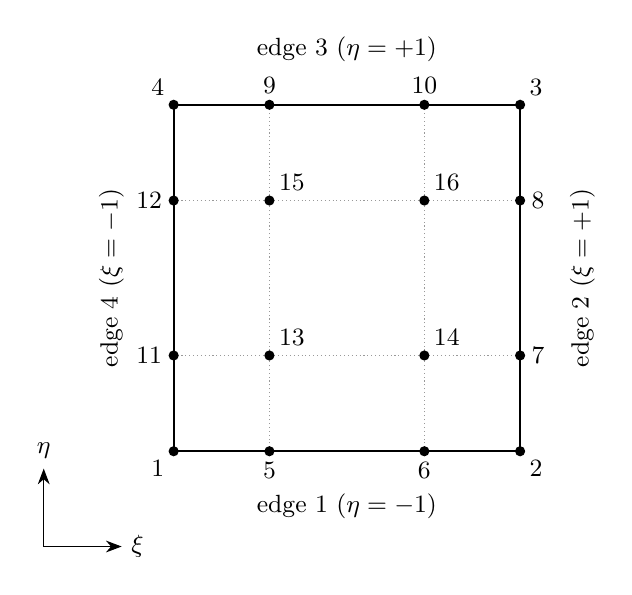
\begin{tikzpicture}[scale=2.2, every node/.style={font=\small},
                    num/.style={inner sep=1.5pt}]
  \def\g{0.4472136}
  % element and node lines
  \draw[thick] (-1,-1) rectangle (1,1);
  \foreach \c in {-\g,\g} {
    \draw[densely dotted, black!40] (\c,-1) -- (\c,1);
    \draw[densely dotted, black!40] (-1,\c) -- (1,\c);
  }
  % nodes: (xi, eta, number, label position); labels of boundary nodes
  % point outwards, labels of interior nodes to the upper right
  \foreach \x/\y/\n/\pos in {
      -1/-1/1/below left, 1/-1/2/below right, 1/1/3/above right, -1/1/4/above left,
      -\g/-1/5/below, \g/-1/6/below,
      1/-\g/7/right, 1/\g/8/right,
      -\g/1/9/above, \g/1/10/above,
      -1/-\g/11/left, -1/\g/12/left,
      -\g/-\g/13/above right, \g/-\g/14/above right,
      -\g/\g/15/above right, \g/\g/16/above right} {
    \node[node dot] at (\x,\y) {};
    \node[num, \pos=2.5pt] at (\x,\y) {\n};
  }
  % edge labels (outside the node numbers)
  \node at (0,-1.32) {edge 1 ($\eta=-1$)};
  \node[rotate=90] at (1.36,0) {edge 2 ($\xi=+1$)};
  \node at (0,1.32) {edge 3 ($\eta=+1$)};
  \node[rotate=90] at (-1.36,0) {edge 4 ($\xi=-1$)};
  % local coordinate axes
  \draw[dimarrow] (-1.75,-1.55) -- (-1.3,-1.55) node[right] {$\xi$};
  \draw[dimarrow] (-1.75,-1.55) -- (-1.75,-1.1) node[above] {$\eta$};
\end{tikzpicture}

  \caption{Local node numbering of a spectral element of degree $p=3$ (GLL nodes).}
  \label{fig:nodes}
\end{figure}

\section{Metric (trial) shape functions in skew coordinates}

\code{ShapeFunctions2D_Metric(xQ, yQ, xN, yN, p)} builds shape functions that
are interpolatory at the element nodes $(x_k,y_k)$ in physical space, in four
steps:
\begin{enumerate}
  \item \textbf{Skew coordinates} (\code{CorotationalSkewCoordinates},
    \cite{Xie2016Modified}; \cite{Yuan1993New}). The skew coordinates $(s,t)$
    are Cartesian coordinates measured along the two element axes at the element
    centre, scaled with the element size: with the centre
    $\vect x_0 = \vect x(0,0)$ and the Jacobian $\matr J_0$ there,
    \begin{equation}
      \begin{bmatrix} s\\ t\end{bmatrix} = \matr J_0^{-\T}\,(\vect x - \vect x_0).
    \end{equation}
    They are linear in $x$ and $y$, move and rotate with the element, and
    coincide with $(\xi,\eta)$ on a parallelogram.
  \item \textbf{Polynomial space.} The shape functions are polynomials of degree
    $p_\upxi$ in $s$ and $p_\upeta$ in $t$ (all products $s^a t^b$ with $a\le
    p_\upxi$, $b\le p_\upeta$, the space $\mathcal Q_p(s,t)$). For good conditioning they
    are written in a Lagrange basis $\ell_a(\tilde s)\,\ell_b(\tilde t)$, where
    $\tilde s$, $\tilde t$ are the skew coordinates scaled to the interval
    $[-1,1]$ of the nodes; the shape functions themselves do not depend on the
    basis (\cref{ch:metric-basis}).
  \item \textbf{Interpolation.} The coefficients follow from the conditions
    $M_j(\vect x_k) = \delta_{jk}$ at the nodes, a linear system with the
    generalized Vandermonde matrix $\matr V$ (values of the basis at the nodes).
  \item \textbf{Derivatives.} The derivatives with respect to $x$ and $y$
    follow from those with respect to $s$ and $t$ with the constant matrix
    $\matr J_0^{-1}$.
\end{enumerate}
Properties (all covered by \code{tests/unit/MetricShapeFunctionsTest.m}):
\begin{itemize}
  \item \textbf{Completeness.} $s$ and $t$ are linear in $x$ and $y$, so every
    polynomial of total degree $\le p$ in $(x,y)$ is a polynomial of degree $\le p$
    in $(s,t)$ and is reproduced exactly on any element shape.
  \item \textbf{Frame invariance.} Rigid-body motions and uniform scaling of the
    element do not change the shape functions.
  \item \textbf{Affine elements.} On a parallelogram the metric and the
    parametric functions coincide, so the element is the classical spectral
    element and $\matr K_e$ is symmetric.
  \item \textbf{Unisolvence.} The interpolation conditions can be singular for
    special node positions on strongly distorted elements, e.g.\ when two nodes
    coincide \parencite{Ooi2008Remedies}. The code stops with an error in this
    case (\code{CheckUnisolvent}), and the studies report such elements as
    rejected.
\end{itemize}

\code{method=2} (\code{p.metricMethod=2}) uses the hybrid space instead of
$\mathcal Q_p(s,t)$: all polynomials of total degree $\le m=\min(p_\upxi,p_\upeta)$ in
the scaled skew coordinates $(\tilde s,\tilde t)$, $\mathcal P_m(\tilde s,\tilde t)$,
complemented by parametric functions of $(\xi,\eta)$
(\cref{sec:metric-hybrid}). It has the same
completeness and invariance, equals the parametric space on all straight-edged
elements and avoids the exponential growth of the Lebesgue constant of
$\mathcal Q_p(s,t)$ on distorted elements.

\section{Element stiffness matrix}

The Jacobian is used in the convention (\code{Jacobi_Matrix})
\begin{equation}
  \matr J = \begin{bmatrix} \partial x/\partial\xi & \partial y/\partial\xi\\
                            \partial x/\partial\eta & \partial y/\partial\eta
            \end{bmatrix}.
\end{equation}
The stiffness matrix (\code{Ke_2D}, vectorized in
\code{studies/thick_cylinder/matlab/cyl_Ke_PM.m}) reads
\begin{equation}
  \matr K_e = \int\limits^{1}_{-1}\int\limits^{1}_{-1}\matr B_\mathrm{L}^{\T}\matr C\,
  \matr B_\mathrm{R}\,\det(\matr J)\dd\xi\dd\eta,
\end{equation}
where $\matr B_\mathrm{L}$ holds the derivatives of the parametric (test) and
$\matr B_\mathrm{R}$ those of the metric (trial) functions. The product
$\det(\matr J)\,\matr B_\mathrm{L}$ is computed with the adjugate of $\matr J$,
$\det(\matr J)\,\matr J^{-1}$, so $\det(\matr J)$ never appears in a
denominator; this is Rajendran's third condition for distortion immunity.
$\matr B_\mathrm{R}$ is evaluated at the physical positions of the Gauss points.
Consequences:
\begin{itemize}
  \item Rigid-body modes lie in both the right and the left null space of
    $\matr K_e$, and $\operatorname{rank}(\matr K_e) = n_\mathrm{dof}-3$, where
    $n_\mathrm{dof}$ is the number of DOFs of the element.
  \item $\matr K_e$ is unsymmetric unless the element is a parallelogram.
\end{itemize}

\subsection*{Numerical integration}
\label{sec:quadrature}

\code{Ke_2D} uses $2p_\upxi\times2p_\upeta$ Gauss-Legendre points by default (other
numbers can be passed); the mesh-level studies of the paper use calibrated rules
(\code{manuscript/studies/ms_rule.m}). Whether a rule integrates the element matrix
exactly depends on the element shape, because the metric functions are polynomials
in $(x,y)$, and $x$, $y$ and $\det(\matr J)$ are polynomials in $(\xi,\eta)$ whose
degree grows with the distortion. The integrands of the trial space
$\mathcal Q_p(s,t)$ are polynomials in $(\xi,\eta)$, so a finite Gauss rule is exact;
its size was determined numerically (smallest rule that reproduces the matrix of a
40-point rule to $10^{-12}$, single elements of \cref{fig:test-elements}):
\begin{center}
  \begin{tabular}{@{}lcc@{}}
    \toprule
    element (input mesh) & $\matr K_e$ exact with & $2p$ sufficient? \\
    \midrule
    parallelogram & $p+1$ & yes \\
    straight edges (4-node) & $\lceil 3p/2\rceil$ & yes \\
    curved edges (8-node), $p\ge2$ & $2p+1$ to $2p+2$ & no \\
    \bottomrule
  \end{tabular}
\end{center}
\begin{figure}[htbp]
  \centering
  % Single test elements (tests/helpers/usemTestElement.m); generated
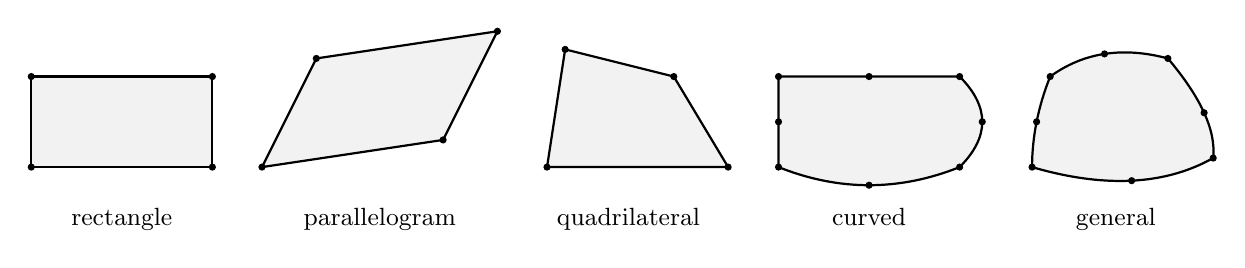
\begin{tikzpicture}[x=1.15cm, y=1.15cm, every node/.style={font=\small}]
  \begin{scope}[xshift=0.00cm]
    \draw[thick, fill=black!5] (0.0000,0.0000) -- (2.0000,0.0000) -- (2.0000,1.0000) -- (0.0000,1.0000) -- cycle;
    \fill (0.0000,0.0000) circle (1.3pt);
    \fill (2.0000,0.0000) circle (1.3pt);
    \fill (2.0000,1.0000) circle (1.3pt);
    \fill (0.0000,1.0000) circle (1.3pt);
    \node[below] at (1.000,-0.35) {rectangle};
  \end{scope}
  \begin{scope}[xshift=2.93cm]
    \draw[thick, fill=black!5] (0.0000,0.0000) -- (2.0000,0.3000) -- (2.6000,1.5000) -- (0.6000,1.2000) -- cycle;
    \fill (0.0000,0.0000) circle (1.3pt);
    \fill (2.0000,0.3000) circle (1.3pt);
    \fill (2.6000,1.5000) circle (1.3pt);
    \fill (0.6000,1.2000) circle (1.3pt);
    \node[below] at (1.300,-0.35) {parallelogram};
  \end{scope}
  \begin{scope}[xshift=6.55cm]
    \draw[thick, fill=black!5] (0.0000,0.0000) -- (2.0000,0.0000) -- (1.4000,1.0000) -- (0.2000,1.3000) -- cycle;
    \fill (0.0000,0.0000) circle (1.3pt);
    \fill (2.0000,0.0000) circle (1.3pt);
    \fill (1.4000,1.0000) circle (1.3pt);
    \fill (0.2000,1.3000) circle (1.3pt);
    \node[below] at (0.900,-0.35) {quadrilateral};
  \end{scope}
  \begin{scope}[xshift=9.49cm]
    \draw[thick, fill=black!5] (0.0000,0.0000) .. controls (0.6667,-0.2667) and (1.3333,-0.2667) .. (2.0000,0.0000) .. controls (2.3333,0.3333) and (2.3333,0.6667) .. (2.0000,1.0000) .. controls (1.3333,1.0000) and (0.6667,1.0000) .. (0.0000,1.0000) .. controls (0.0000,0.6667) and (0.0000,0.3333) .. (0.0000,0.0000) -- cycle;
    \fill (0.0000,0.0000) circle (1.3pt);
    \fill (2.0000,0.0000) circle (1.3pt);
    \fill (2.0000,1.0000) circle (1.3pt);
    \fill (0.0000,1.0000) circle (1.3pt);
    \fill (1.0000,-0.2000) circle (1.3pt);
    \fill (2.2500,0.5000) circle (1.3pt);
    \fill (1.0000,1.0000) circle (1.3pt);
    \fill (0.0000,0.5000) circle (1.3pt);
    \node[below] at (1.000,-0.35) {curved};
  \end{scope}
  \begin{scope}[xshift=12.71cm]
    \draw[thick, fill=black!5] (0.0000,0.0000) .. controls (0.8000,-0.2333) and (1.4667,-0.2000) .. (2.0000,0.1000) .. controls (2.0333,0.4000) and (1.8667,0.7667) .. (1.5000,1.2000) .. controls (1.0000,1.3333) and (0.5667,1.2667) .. (0.2000,1.0000) .. controls (0.0667,0.6667) and (0.0000,0.3333) .. (0.0000,0.0000) -- cycle;
    \fill (0.0000,0.0000) circle (1.3pt);
    \fill (2.0000,0.1000) circle (1.3pt);
    \fill (1.5000,1.2000) circle (1.3pt);
    \fill (0.2000,1.0000) circle (1.3pt);
    \fill (1.1000,-0.1500) circle (1.3pt);
    \fill (1.9000,0.6000) circle (1.3pt);
    \fill (0.8000,1.2500) circle (1.3pt);
    \fill (0.0500,0.5000) circle (1.3pt);
    \node[below] at (0.925,-0.35) {general};
  \end{scope}
\end{tikzpicture}

  \caption{Single test elements of the element tests, of the element studies of the
    paper and of the table on numerical integration
    (\texttt{usemTestElement}): the rectangle $[0,2]\times[0,1]$
    (\texttt{'square'}), a parallelogram, a quadrilateral with straight,
    non-parallel edges (\texttt{'trapezoid'}), and two 8-node elements with
    curved edges.
    The dots are the nodes of the input element; the spectral element of degree
    $p$ is generated from them.}
  \label{fig:test-elements}
\end{figure}

For straight edges the numbers follow from the polynomial degrees: $x$ and $y$
are linear in $\xi$ and in $\eta$, so $s^a t^b$ has degree up to $2p$ in each
direction. On curved elements, the degrees double because $x$ and $y$ are
quadratic, and $2p$ points under-integrate the matrix
(\textcite{Eisentraeger2025unsymmetric} discuss the numerical integration of
unsymmetric elements in detail).

The exactness of the patch tests is not affected: a polynomial displacement field
of degree $\le p$ produces stresses of degree $\le p-1$ in $(x,y)$, and the
integrand of the corresponding stiffness terms has degree $\le 3p-1$ per
direction even on curved elements, which $2p$ points integrate exactly. This is
why the patch tests of \cref{ch:testing} are passed to machine precision on all
meshes. For the hybrid space (\code{method = 2}), the gradients of the
parametric part contain $\matr J^{-1}$, so the stiffness integrand is a rational
function on non-affine elements and no Gauss rule integrates it exactly.

\paragraph{Loads and errors.} Edge tractions and body loads are integrated with
the parametric (test) functions (\code{cyl_loads}, \code{rp_loads}), consistent with
the weak form \eqref{eq:weakform}. Displacements and strains inside the elements
are evaluated with the trial functions (\code{cyl_errors}).

\paragraph{Linear solver.} $\matr K$ is unsymmetric, so the studies use LU
decomposition (\texttt{MATLAB}'s \texttt{\textbackslash}), not Cholesky.

\chapter{Basis of the metric Vandermonde matrix}
\label{ch:metric-basis}

% Line colours of the plots in this chapter (monomial, Legendre, Chebyshev,
% Lagrange, ...)
\pgfplotscreateplotcyclelist{metricbasis}{%
  red\\blue\\black\\green!50!black\\orange\\violet\\}

The metric (trial) shape functions are computed from a generalized Vandermonde
matrix, i.e.\ from the values of a set of basis polynomials at the element nodes
(\cref{ch:theory}). Any basis of the polynomial space can be used for this
purpose. This chapter summarizes the implementation of the four bases compared in
the paper and of the hybrid trial space (\code{method=2}). The results are those of
\code{manuscript/studies/ms_element_study.m} (data:
\code{manuscript/data/element-*.dat}); the discussion is given in the paper. The
tests are in \code{tests/unit/MetricBasisTest.m} and
\code{tests/unit/MetricHybridTest.m}.

\section{Setting and basis invariance}

An element of degree $(p_\upxi,p_\upeta)$ has $n=(p_\upxi+1)(p_\upeta+1)$ nodes
$\vect x_k$ with skew coordinates $(s_k,t_k)$. Its metric shape functions $M_l$,
$l=1,\dots,n$, are polynomials of the space $\mathcal Q_p(s,t)$ (degree $p_\upxi$ in $s$
and $p_\upeta$ in $t$, \cref{ch:theory}) and are interpolatory,
$M_l(\vect x_k)=\delta_{lk}$. To compute them, the code takes $n$ basis
polynomials $\phi_c$ of $\mathcal Q_p(s,t)$, evaluates them at the nodes,
$V_{ck}=\phi_c(\vect x_k)$, and at the query points (Gauss points),
$P_{cq}=\phi_c(\vect x_q)$, and solves
\[
  \matr V\,\matr N=\matr P,\qquad N_{lq}=M_l(\vect x_q).
\]

\paragraph{The basis does not change the shape functions.} If $\matr V$ is
non-singular, $\mathcal Q_p(s,t)$ contains exactly one set of functions with the
Kronecker property $M_l(\vect x_k)=\delta_{lk}$, so every basis leads to the same
$M_l$. (A change of basis multiplies $\matr V$ and $\matr P$ from the left with
the same non-singular matrix, which cancels in $\matr V^{-1}\matr P$.)

\paragraph{The basis changes the round-off error.} The system is solved by an LU
decomposition with partial pivoting. The relative error of the computed shape
functions is then bounded, up to a modest factor that depends on $n$, by
$\kappa(\matr V)\,\epsilon$, where $\epsilon\approx1.1\times10^{-16}$ is the unit
round-off of double precision \parencite{Higham2002Accuracy}. Roughly speaking,
every decade of the condition number $\kappa(\matr V)$ costs one significant
digit.

\section{Bases}

\code{PolynomialBasis1D(s, n, basis)} provides, for the polynomial
degree $p$ (argument \code{n}), with values and first derivatives,
\begin{center}
  \begin{tabularx}{\linewidth}{@{}lL@{}}
    \toprule
    \code{basis} & $\phi_a(s)$, $a=0,\dots,p$ \\
    \midrule
    \code{'monomial'} & $s^a$ (used without scaling) \\
    \code{'legendre'} & Legendre polynomials $L_a(s)$, three-term recurrence \\
    \code{'chebyshev'} & Chebyshev polynomials $T_a(s)$, three-term recurrence \\
    \code{'lagrange'} & Lagrange polynomials $\ell_a(s)$ through the 1D reference
      nodes \code{nodal_distribution(n)}, product formula (no division by
      the differences $s-s_m$ to the nodes $s_m$, so query points may coincide
      with nodes) \\
    \bottomrule
  \end{tabularx}
\end{center}
The 2D basis is the tensor product $\phi_a(\tilde s)\,\phi_b(\tilde t)$. The
Legendre, Chebyshev and Lagrange bases are defined on $[-1,1]$, but on distorted
elements the skew coordinates of the nodes leave $[-1,1]^2$. Outside $[-1,1]$ these
polynomials grow quickly. For these three bases \code{ShapeFunctions2D_Metric}
therefore maps the bounding box of the nodes in $(s,t)$ onto $[-1,1]^2$,
\begin{equation}
  \tilde s = (s-c_\mathrm{s})/r_\mathrm{s},\qquad
  \tilde t = (t-c_\mathrm{t})/r_\mathrm{t},
\end{equation}
where $(c_\mathrm{s},c_\mathrm{t})$ is the centre and $(r_\mathrm{s},r_\mathrm{t})$
are the half widths of the box. The map is affine and computed from
frame-invariant quantities, so the space $\mathcal Q_p$ and the frame invariance are
preserved; on a parallelogram it is the identity. The monomial basis is used
without this scaling. The basis is selected with \code{p.metricBasis} (default
\code{'lagrange'}).

\Cref{fig:metric-basis-kappa,fig:metric-basis-leb} show the conditioning and the
Lebesgue constants. On a parallelogram, the Lagrange basis gives $\kappa_2(\matr V)=1$
for every $p$, since $\matr V$ is then a permutation matrix. On distorted elements,
the three scaled bases are close to one another, and the Lebesgue constant of
$\mathcal Q_p(s,t)$ grows exponentially with $p$. Since the shape functions do not
depend on the basis, no basis can remove this growth.

\begin{figure}[htbp]
  \centering
  \begin{tikzpicture}
    \begin{groupplot}[group style={group size=2 by 2, horizontal sep=2.6cm,
        vertical sep=2.2cm}, width=0.44\linewidth, height=0.35\linewidth,
        ymode=log, grid=major, xlabel={$p$}, ylabel={$\kappa_2(\matr V)$},
        ymin=0.5, ymax=1e16, xmin=1, xmax=16, cycle list name=metricbasis,
        unbounded coords=discard,
        every axis plot/.append style={mark size=1.4pt}]
      \nextgroupplot[title={parallelogram},
        legend to name=leg:metricbasis, legend columns=4,
        legend style={font=\footnotesize}]
      \addplot+[mark=*] table[x=p, y=kappa2_mon]{../manuscript/data/element-parallelogram.dat};
      \addplot+[mark=square*] table[x=p, y=kappa2_leg]{../manuscript/data/element-parallelogram.dat};
      \addplot+[mark=triangle*] table[x=p, y=kappa2_che]{../manuscript/data/element-parallelogram.dat};
      \addplot+[mark=diamond*] table[x=p, y=kappa2_lag]{../manuscript/data/element-parallelogram.dat};
      \legend{monomial, Legendre, Chebyshev, Lagrange}
      \nextgroupplot[title={quadrilateral}]
      \addplot+[mark=*] table[x=p, y=kappa2_mon]{../manuscript/data/element-trapezoid.dat};
      \addplot+[mark=square*] table[x=p, y=kappa2_leg]{../manuscript/data/element-trapezoid.dat};
      \addplot+[mark=triangle*] table[x=p, y=kappa2_che]{../manuscript/data/element-trapezoid.dat};
      \addplot+[mark=diamond*] table[x=p, y=kappa2_lag]{../manuscript/data/element-trapezoid.dat};
      \nextgroupplot[title={curved}]
      \addplot+[mark=*] table[x=p, y=kappa2_mon]{../manuscript/data/element-curved.dat};
      \addplot+[mark=square*] table[x=p, y=kappa2_leg]{../manuscript/data/element-curved.dat};
      \addplot+[mark=triangle*] table[x=p, y=kappa2_che]{../manuscript/data/element-curved.dat};
      \addplot+[mark=diamond*] table[x=p, y=kappa2_lag]{../manuscript/data/element-curved.dat};
      \nextgroupplot[title={general}]
      \addplot+[mark=*] table[x=p, y=kappa2_mon]{../manuscript/data/element-general.dat};
      \addplot+[mark=square*] table[x=p, y=kappa2_leg]{../manuscript/data/element-general.dat};
      \addplot+[mark=triangle*] table[x=p, y=kappa2_che]{../manuscript/data/element-general.dat};
      \addplot+[mark=diamond*] table[x=p, y=kappa2_lag]{../manuscript/data/element-general.dat};
    \end{groupplot}
  \end{tikzpicture}\\[4pt]
  \ref{leg:metricbasis}
  \caption{Condition number of the metric Vandermonde matrix on the single test
    elements of \cref{fig:test-elements} (bounding-box scaling for the Legendre,
    Chebyshev and Lagrange bases).}
  \label{fig:metric-basis-kappa}
\end{figure}

\section{Hybrid trial space (\texttt{method=2})}
\label{sec:metric-hybrid}

\paragraph{Definition.} With $m=\min(p_\upxi,p_\upeta)$ and the Legendre
polynomials $L_a$, the hybrid trial space is
\begin{equation}
  \mathcal T_p = \mathcal P_m(\tilde s,\tilde t)\;\oplus\;\operatorname{span}\{L_a(\xi)L_b(\eta):\
  a\le p_\upxi,\ b\le p_\upeta,\ a+b>m\}.
  \label{eq:hybrid-space}
\end{equation}
The first part, $\mathcal P_m(\tilde s,\tilde t)$, consists of all polynomials of total
degree $\le m$ in the bounding-box scaled skew coordinates $(\tilde s,\tilde t)$;
the code spans it with the products $L_a(\tilde s)L_b(\tilde t)$, $a+b\le m$.
Because $\tilde s$ and $\tilde t$ are affine functions of $x$ and $y$, and vice
versa, $\mathcal P_m(\tilde s,\tilde t)=\mathcal P_m(x,y)$. The hybrid space therefore
contains all complete polynomials of degree $m$ in $x$ and $y$ and, since
$(\tilde s,\tilde t)$ move and rotate with the element, it is frame invariant. The
second part, the complement, is written in the parametric coordinates $(\xi,\eta)$,
in which the element nodes form a tensor grid. On non-affine elements the complement
depends on the polynomials used. The Legendre basis is therefore part of the
definition, and \code{p.metricBasis} is ignored for \code{method=2}.

\paragraph{Straight-edged elements.} If the geometry map is bilinear and the
hybrid Vandermonde matrix is non-singular, the hybrid space equals the
parametric space, $\mathcal T_p=\mathcal Q_p(\xi,\eta)$: the metric functions coincide with the
parametric ones, and the element is the classical (symmetric) spectral element.
The reason is that $x$ and $y$ are bilinear in $(\xi,\eta)$ for such a map, so a
polynomial of total degree $\le m$ in $x$ and $y$ has degree $\le m$ in $\xi$ and
in $\eta$ \parencite[cf.][]{Arnold2002Approximation}.

\paragraph{Folded and inverted elements.} The hybrid functions are evaluated only
through $(\xi,\eta)$, so the sign of $\det(\matr J)$ is irrelevant, and completeness
holds pointwise in $(\xi,\eta)$, also where the map folds. Only $\det(\matr J)=0$ at
an evaluation point is excluded, because the gradients of the complement contain
$\matr J^{-1}$ (error \code{ShapeFunctions2D_Metric:singularJacobian}).

\paragraph{Implementation.} The hybrid space is selected with
\code{p.metricMethod=2} or for a single call with
\code{ShapeFunctions2D_Metric(..., p, 2, xiQ)}. The parametric coordinates of the
nodes are the reference nodes (\code{ReferenceNodes2D}). Those of the query points
are passed by the callers, which evaluate at mapped quadrature or sampling points.
The gradients of $\mathcal P_m(\tilde s,\tilde t)$ follow from the constant matrix
$\matr J_0^{-1}$ of the skew coordinates, those of the complement from the Jacobian
at the query point, $\nabla_{\vect x}\phi=\matr J^{-1}\nabla_{\xi}\phi$.

\begin{figure}[htbp]
  \centering
  \begin{tikzpicture}
    \begin{semilogyaxis}[width=0.62\linewidth, height=0.42\linewidth,
        xlabel={$p$}, ylabel={Lebesgue constant}, grid=major, ymax=1e12,
        legend cell align=left, legend style={font=\footnotesize, at={(0.02,0.98)}, anchor=north west},
        cycle list name=metricbasis]
      \addplot+[mark=square*] table[x=p, y=LQ]{../manuscript/data/element-trapezoid.dat};
      \addplot+[mark=triangle*] table[x=p, y=LQ]{../manuscript/data/element-general.dat};
      \addplot+[mark=o] table[x=p, y=LQ]{../manuscript/data/element-curved.dat};
      \addplot+[mark=square, dashed] table[x=p, y=LT]{../manuscript/data/element-trapezoid.dat};
      \addplot+[mark=triangle, dashed] table[x=p, y=LT]{../manuscript/data/element-general.dat};
      \addplot+[mark=x, dashed] table[x=p, y=LT]{../manuscript/data/element-curved.dat};
      \legend{{$\mathcal Q_p(s,t)$ quadrilateral}, {$\mathcal Q_p(s,t)$ general}, {$\mathcal Q_p(s,t)$ curved},
              $\mathcal T_p$ quadrilateral, $\mathcal T_p$ general, $\mathcal T_p$ curved}
    \end{semilogyaxis}
  \end{tikzpicture}
  \caption{Lebesgue constant of the metric interpolation in $\mathcal Q_p(s,t)$
    (\texttt{method=1}) and in the hybrid space $\mathcal T_p$ (\texttt{method=2}) on
    the distorted test elements of \cref{fig:test-elements}.}
  \label{fig:metric-basis-leb}
\end{figure}

\chapter{Getting started}
\label{ch:start}

\section{Requirements}

\begin{xltabular}{\linewidth}{@{}P{5.2cm}L@{}}
  \toprule
  Product & needed for \\
  \midrule
  MATLAB R2018b or newer (developed and tested with R2026a) & everything \\
  Parallel Computing Toolbox (optional) & \code{Start_Sim.m} opens a parallel
    pool if the toolbox is available; otherwise the \code{parfor} loops run
    serially \\
  Symbolic Math Toolbox & \code{MMS_2D} (manufactured solutions),
    \code{HigherOrderDisplacementField.m}, Padé helpers \\
  Signal Processing Toolbox & \code{FFT_Signal} with \code{SignalType = 5}
    (\code{findpeaks}) \\
  Optimization Toolbox & \code{Global2LocalCoordinatesQuad} (\code{fsolve}), not
    used in the main flow \\
  Deep Learning Toolbox & \code{combvec} in the Q8 branch of \code{distort_mesh}
    / \code{distort_single_element} \\
  \bottomrule
\end{xltabular}
The test suite needs only base MATLAB.

\section{Running a simulation}

\begin{enumerate}
  \item Change the MATLAB current folder to \code{code/}; all paths in
    \code{Start_Sim.m} are relative to it.
  \item Choose an input file in \code{Start_Sim.m} (\code{filename = ...}). The
    ABAQUS input files in \code{code/InputFilesAbaqus} are found through the
    MATLAB path:
    \begin{center}
      \begin{tabularx}{0.95\linewidth}{@{}lL@{}}
        \toprule
        file & test \\
        \midrule
        \code{PatchTestLeeQuadratic_*.inp} & Lee \& Bathe quadratic patch test
          (pure bending); undistorted, angular, mid-edge \\
        \code{PatchTestLeeCubic_*.inp} & Lee \& Bathe cubic patch test;
          undistorted, angular, mid-edge \\
        \code{PatchTestLeeCubic_Rajendran_adj.inp} & cubic test on five distorted
          8-node elements \\
        \bottomrule
      \end{tabularx}
    \end{center}
  \item Set the parameters (\cref{sec:parameters}) and run \code{Start_Sim}:
\begin{lstlisting}
cd code
Start_Sim
\end{lstlisting}
\end{enumerate}
\code{Start_Sim} clears the workspace, sets \code{dbstop if error}, deletes
\code{subroutines/Temp/*.mat}, reads the input file, lifts the mesh to degree
$p$ and calls one of the analysis scripts (\code{call_Static},
\code{call_Dynamic}, \code{call_Modal}, \code{call_FrequencyDomain}). They are
scripts, not functions, so all variables stay in the base workspace.

\section{Parameters in \texttt{Start\_Sim.m}}
\label{sec:parameters}

\begin{xltabular}{\linewidth}{@{}P{5.2cm}L@{}}
  \toprule
  variable & meaning \\
  \midrule
  \endhead
  \code{filename} & ABAQUS input file (\code{.inp}, without path) \\
  \code{analysis_type} & \code{'Static_analysis'}, \code{'Dynamic_analysis'},
    \code{'Modal_analysis'}, \code{'FrequencyDomain_analysis'} \\
  \code{saveWS} & save the workspace to \code{subroutines/Results/...} \\
  \code{plot_mesh}, \code{plot_disp}, \code{plot_stress}, \code{plot_strain} & plots \\
  \code{antype} & 1 = plane stress, 2 = plane strain \\
  \code{p.pxi}, \code{p.peta} & polynomial degree in $\xi$ and $\eta$; if the local
    coordinate systems of neighbouring elements are not aligned, both are set to
    the minimum \\
  \code{p.ndist} & node distribution (1 equidistant, 2 GLL, 3 GLC) \\
  \code{mass_matrix} & 1 consistent, 2 nodal quadrature (GLL), 3 row-sum, 4 HRZ \\
  \code{flag_mRHS} & dynamic analysis: one right-hand side per load case; if
    true, only the central difference (\code{Method < 300}) or HHT-$\alpha$
    (\code{Method >= 300}) solvers are used \\
  \code{omega_vec}, \code{zeta_vec} & Rayleigh damping: two angular frequencies
    [rad/s] and damping ratios \\
  \code{numEigen}, \code{EVP_Solver.*} & modal analysis (\code{eigs} options) \\
  \code{SignalType}, \code{ExciteParam} & time signal of time-dependent loads
    (\cref{sec:signals}) \\
  \code{save_var} & dynamic analysis: 0 = save only the nodes of interest (DOF 6
    in the input file), 1 = all DOFs \\
  \code{TimeIntegration.Method} & time integration scheme (\cref{tab:methods}) \\
  \code{TimeIntegration.Order}, \code{.rho}, \code{.dtImp}, \code{.nInterp},
    \code{.SolverSave} & options of the time integrators \\
  \code{fHarmonic} & excitation frequency of the frequency-domain analysis [Hz] \\
  \bottomrule
\end{xltabular}

\section{Output}

\begin{center}
  \begin{tabularx}{\linewidth}{@{}lL@{}}
    \toprule
    analysis & results file \\
    \midrule
    static & \code{subroutines/Results/Static/<name>_Static/<name>_ndof<N>.mat} \\
    dynamic & \code{subroutines/Results/Dynamic/<name>_<Method>/<name>_ndof<N>_<mass>.mat} \\
    modal & \code{subroutines/Results/Modal/<name>_Modal/<name>_ndof<N>_<mass>.mat} \\
    frequency domain & \code{subroutines/Results/Frequency_Domain/<name>_Frequency_Domain/...} \\
    \bottomrule
  \end{tabularx}
\end{center}
These folders are excluded from version control. The most important variables
of a saved workspace:
\begin{center}
  \begin{tabularx}{\linewidth}{@{}lL@{}}
    \toprule
    variable & content \\
    \midrule
    \code{Topology_Node}, \code{xCoor}, \code{yCoor} & spectral element mesh \\
    \code{K}, \code{M}, \code{R} & stiffness, mass, damping (sparse, after the
      Dirichlet conditions) \\
    \code{F} & load vector \\
    \code{u}, \code{ux}, \code{uy} & static displacements \\
    \code{EF}, \code{U} & eigenfrequencies and mode shapes (modal analysis) \\
    \code{t_comp}, \code{y_comp} & time and displacement history (dynamic analysis) \\
    \bottomrule
  \end{tabularx}
\end{center}

\section{Using the building blocks without \texttt{Start\_Sim}}

The test helpers show how to use the routines directly:
\begin{lstlisting}
addpath(genpath('code/subroutines')); addpath('tests/helpers');

% 3 x 2 mesh of 8-node elements with curved edges, lifted to p = 4
[nodes, topo] = usemTestMesh(3, 2, 3, 2, 2);
nodes = usemDistortMesh(nodes, topo, 'combined', 0.3);
model = usemBuildModel(nodes, topo, 4);          % GLL nodes

% unsymmetric stiffness matrix (plane stress, E = 1, nu = 0.3)
K = usemAssemble(model, HookeMatrix2d(1, 0.3, 1));

% displacement patch test with the field u = (Re z^4, -Im z^4)
field = @(x, y) deal(real((x + 1i*y).^4), -imag((x + 1i*y).^4));
[u, uExact, err] = usemDirichletSolve(K, model, field);   % err ~ 1e-15
\end{lstlisting}
\code{usemReadAbaqus(inpFile, p)} runs the input part of \code{Start_Sim.m}
(reading and lifting to degree $p$) and returns the model as a struct.

\chapter{ABAQUS input files}
\label{ch:input}

The model is defined in an ABAQUS/CAE input file (\code{*.inp}). The readers in
\code{subroutines/ReadInputFileAbaqus} are not a general ABAQUS parser. They
expect the structure that ABAQUS/CAE writes, including several of its comment
lines. The safest approach is to build the model in ABAQUS/CAE (one part, one
instance, 2D planar, CPS4/CPE4 or CPS8/CPE8 elements) and to start from one of
the examples in \code{code/InputFilesAbaqus}.

\section{Reading sequence}

\begin{enumerate}
  \item \code{Adjust_Set_names_input_file_ABAQUS(filename)} writes
    \code{<name>_adjusted.inp} to the current folder. In it, every \code{Set-}
    after \code{End Instance} is renamed to \code{PickedSet-}, and the node/element
    set pairs named \code{Pressure} and \code{Traction} are numbered
    (\code{Pressure1}, \code{Pressure2}, \dots) in order of appearance.
  \item \code{Read_mesh_ABAQUS}: nodes $(x,y)$ and element connectivity.
  \item \code{Read_material_ABAQUS}: materials and their element sets.
  \item \code{Read_step_ABAQUS}: step names, types and the time period of
    \code{*Dynamic} steps.
  \item \code{Read_load_ABAQUS}: concentrated forces, edge loads, body forces and
    gravity.
  \item \code{Read_boundary_condition_ABAQUS}: Dirichlet conditions and nodes of
    interest.
  \item The adjusted file is deleted.
  \item \code{pSpectralElement_NodesTopology} and \code{pSpectralElement_BCs} lift
    the mesh and the edge-based sets to degree $p$.
\end{enumerate}

\section{Requirements and conventions}

\paragraph{Mesh.}
\begin{itemize}
  \item Only the first \code{*Node} block is read, and only $x$ and $y$. Node
    labels must be numbered consecutively from 1 (checked by the reader).
  \item Element types ending in \code{4}/\code{4R} give 4-node elements, types
    containing \code{8} give 8-node elements. One element type per model.
  \item For 8-node meshes the corner nodes must be numbered before the mid-side
    nodes (\code{pSpectralElement_NodesTopology} keeps nodes \code{1..nCorner} and
    stops with an error otherwise).
  \item The element block must be followed directly by \code{*Nset},
    \code{*End Part} or \code{*End Instance}.
\end{itemize}

\paragraph{Sections and materials.}
\begin{itemize}
  \item \code{*Solid Section, elset=<set>, material=<mat>}, preceded by a
    \code{** Section:} comment.
  \item A \code{** MATERIALS} header; the material block ends with the
    \code{** ----} line that CAE writes.
  \item \code{*Density}, \code{*Elastic} (isotropic \code{E, nu},
    \code{ENGINEERING CONSTANTS} or \code{ORTHO}) and \code{*Damping}.
    \code{*Damping} only switches Rayleigh damping on for the element set; the
    parameters come from \code{omega_vec} and \code{zeta_vec}.
\end{itemize}

\paragraph{Sets.}
\begin{itemize}
  \item Sets used by boundary conditions and loads must be defined in the
    \emph{assembly} (after \code{*End Instance}), as CAE does. Otherwise the
    boundary condition reader stops with the error ``Node set \dots\ was not
    found''. Set names are matched exactly (\code{Set-1} is not \code{Set-10}).
  \item Node and element sets with \code{generate} are expanded by the readers
    (also for \code{*Cload}).
  \item Boundary-condition set names must contain \code{Set} (\code{Set-1},
    \code{_PickedSet3}, \dots).
  \item A set on an \emph{edge} needs a node set \emph{and} an element set with the
    same name (CAE creates both when edges are picked). Only then can
    \code{pSpectralElement_BCs} add the high-order nodes of that edge. Point
    constraints only need a node set.
  \item Edge loads: define node set and element set as \code{Pressure} (pressure
    loads) or \code{Traction} (surface tractions), in the order of the loads in
    the step.
\end{itemize}

\paragraph{Step, boundary conditions and loads} (only data after
\code{** STEP:} is read):

\begin{xltabular}{\linewidth}{@{}P{5.6cm}P{2.6cm}L@{}}
  \toprule
  ABAQUS & internal \code{type} & notes \\
  \midrule
  \endhead
  \code{*Boundary} with \code{Set-1, ENCASTRE} or \code{PINNED} & \code{fixed} & $u_x = u_y = 0$ \\
  \code{Set-1, XSYMM} / \code{YSYMM} & \code{XSYMM} / \code{YSYMM} & \\
  \code{Set-1, 1, 1} & \code{Ux 0} & homogeneous \\
  \code{Set-1, 1, 1, 0.001} & \code{Ux} & prescribed value 0.001, applied by elimination \\
  \code{Set-1, 1, 1} and \code{Set-1, 2, 2} (two lines, as CAE writes U1 + U2) & \code{UxUy 0} & \\
  \code{*Boundary, amplitude=...} & \code{Ux dt}, \code{Uy dt} & time-dependent; time function from \code{SignalType} \\
  \code{*Boundary, user} & \code{Ux fx}, \code{Uy fx} & spatially varying, \code{SpatialDisplacementFunction.m} \\
  \code{Set-5, 6, 6} & \code{noi} & node of interest for the output of the dynamic analysis; not a constraint \\
  \code{*Cload}: \code{Set, 1, F} & \code{f_x} / \code{f_y} & full value at every node of the set; \code{amplitude=} gives \code{f_x_dt} \\
  \code{*Dsload}: \code{Pressure, P, p} & \code{Pressure} & along the inward normal \\
  \code{*Dsload}: \code{Pressure, PNU, a} & \code{Pressure fx} & $p(x,y)$ from \code{SpatialLoadingFunction.m} \\
  \code{*Dsload}: \code{Traction, TRVEC, a, dx, dy, dz} & \code{Traction} & traction $a\,(d_x, d_y)$ \\
  \code{*Dsload}: \code{Traction, TRVECNU, a, dx, dy, dz} & \code{Traction fx} & $a\,(d_x, d_y)\,f(x,y)$ from \code{SpatialLoadingFunction.m} \\
  \code{*Dload} with \code{BX}/\code{BY} (CAE comment \code{Body force}) & \code{Body_force} & \\
  \code{*Dload}: \code{..., GRAV, g, dx, dy} & gravity & all elements \\
  \bottomrule
\end{xltabular}

\code{*Amplitude} tables are ignored: the time history of every time-dependent
load is the signal selected by \code{SignalType} in \code{Start_Sim.m}.
\code{SpatialLoadingFunction.m} contains the loads of the Lee \& Bathe cubic
patch test: \code{Pressure fx} gives $a\cdot 120\,y$, \code{Traction fx} gives
$a\,(6 - 6y^2)$.

\section{Data structures returned by the readers}

\begin{xltabular}{\linewidth}{@{}P{4.6cm}L@{}}
  \toprule
  variable & layout \\
  \midrule
  \code{nodes} & \code{[nNodes x 2]} coordinates \\
  \code{topology} & \code{[nElem x 4]} or \code{[nElem x 8]} connectivity \\
  \code{material_properties{i,1:5}} & density, dielectric (legacy), elastic
    constants (\code{[E nu]} or 9 orthotropic stiffness values), piezoelectric
    (legacy), damping \\
  \code{material_elset{i}} & elements of material \code{i} \\
  \code{cload(k)}, \code{dsload(k)} & struct arrays with the fields
    \code{set_name}, \code{amplitude}, \code{type}, \code{nset}, \code{elset},
    \code{DirectionVector}, \code{step_name} (\code{cload} has no \code{elset}
    and no \code{DirectionVector}) \\
  \code{body_force(k)}, \code{gravity(k)} & \code{amplitude = [bx; by]} or
    \code{[g; dx; dy]}, \code{elset} \\
  \code{boundary_conditions(k)} & column struct array with the fields
    \code{set_name}, \code{amplitude}, \code{type}, \code{nset}, \code{elset},
    \code{step_name}, in reverse order of appearance \\
  \bottomrule
\end{xltabular}

\section{Example: Lee \& Bathe quadratic patch test}
\label{sec:leebathe}

The file \code{PatchTestLeeQuadratic_angular.inp} contains a plate
$[0,10]\times[-1,1]$ with two 4-node elements and angular distortion,
$u_x = 0$ on the left edge (\code{Set-1}, node set and element set), $u_y = 0$
at $(0,-1)$ (\code{Set-2}) and the pressure $p = 120\,y$ on the right edge
(\code{Pressure}, \code{PNU}); see \cref{fig:leebathe}. The exact solution is
pure bending (plane stress, $\sigma_x = a y$):
\begin{equation}
  u_x = \frac{a\,x\,y}{E},\qquad
  u_y = -\frac{a}{2E}\left(x^2 + \nu y^2\right) + \frac{a\,\nu}{2E}.
\end{equation}
For $p\ge2$ the unsymmetric spectral element reproduces it to machine precision
on all three meshes (\code{tests/integration/LeeBathePatchTest.m},
\code{tests/integration/AbaqusInputTest.m}).

\begin{figure}[htbp]
  \centering
  % Lee & Bathe (1993) quadratic patch test: plate [0,10] x [-1,1],
% boundary conditions, load and the three meshes of code/InputFilesAbaqus
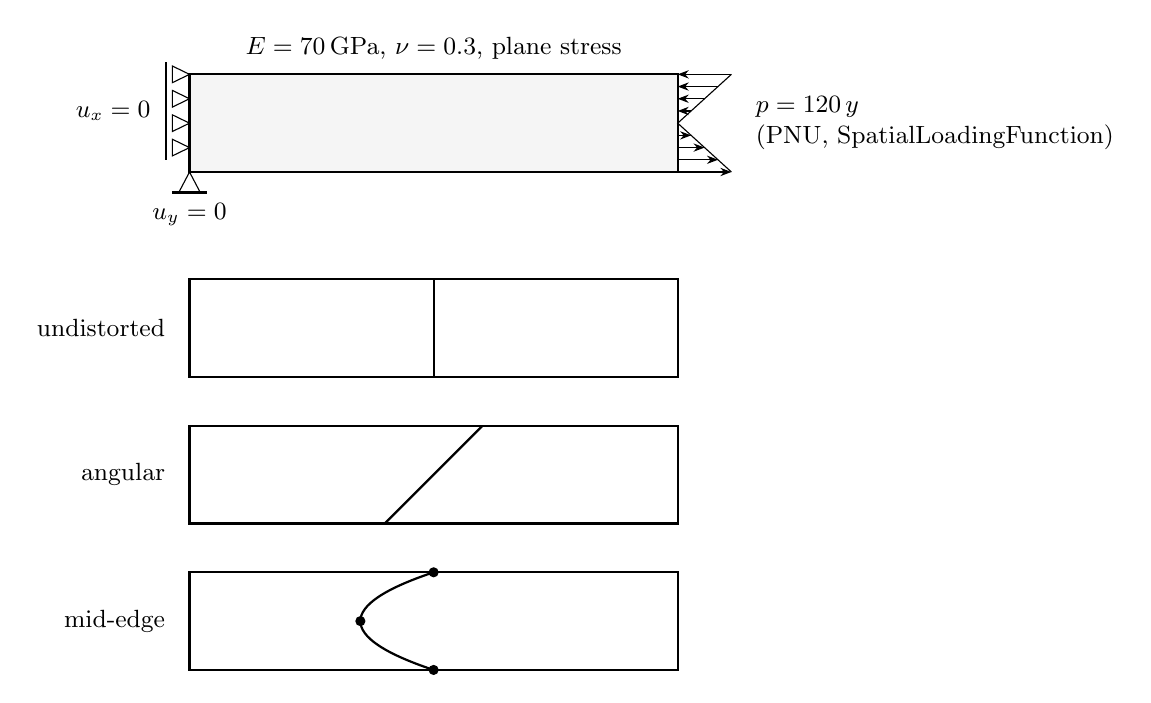
\begin{tikzpicture}[x=0.62cm, y=0.62cm, every node/.style={font=\small}]
  % ---- model with boundary conditions and load ----
  \begin{scope}
    \draw[thick, fill=black!4] (0,-1) rectangle (10,1);
    \node[above=2pt] at (5,1) {$E=70\,\mathrm{GPa}$, $\nu=0.3$, plane stress};
    % u_x = 0 on the left edge: rollers on a vertical wall
    \foreach \y in {-0.5,0,0.5,1} {
      \draw (0,\y) -- (-0.35,\y+0.17) -- (-0.35,\y-0.17) -- cycle;
    }
    \draw[thick] (-0.48,-0.75) -- (-0.48,1.25);
    \node[left] at (-0.6,0.25) {$u_x=0$};
    % u_y = 0 (and u_x = 0) at (0,-1): pin
    \draw (0,-1) -- (-0.22,-1.42) -- (0.22,-1.42) -- cycle;
    \draw[thick] (-0.35,-1.42) -- (0.35,-1.42);
    \node[below] at (0,-1.45) {$u_y=0$};
    % linearly varying pressure p = 120 y on the right edge: compression
    % (pointing inwards) for y > 0, tension (pointing outwards) for y < 0
    \foreach \y in {0.25,0.5,0.75,1} {
      \draw[-{Stealth[length=1.4mm]}] (10+1.1*\y,\y) -- (10,\y);
      \draw[-{Stealth[length=1.4mm]}] (10,-\y) -- (10+1.1*\y,-\y);
    }
    \draw (11.1,1) -- (10,0) -- (11.1,-1);
    \node[right, align=left] at (11.4,0)
      {$p=120\,y$\\(\code{PNU}, \code{SpatialLoadingFunction})};
  \end{scope}
  % ---- meshes (node coordinates of the input files) ----
  \begin{scope}[shift={(0,-4.2)}]
    \draw[thick] (0,-1) rectangle (10,1);
    \draw[thick] (5,-1) -- (5,1);
    \node[left] at (-0.3,0) {undistorted};
  \end{scope}
  \begin{scope}[shift={(0,-7.2)}]
    \draw[thick] (0,-1) rectangle (10,1);
    \draw[thick] (4,-1) -- (6,1);
    \node[left] at (-0.3,0) {angular};
  \end{scope}
  \begin{scope}[shift={(0,-10.2)}]
    \draw[thick] (0,-1) rectangle (10,1);
    % parabolic edge through (5,1), (3.5,0), (5,-1): quadratic Bezier with
    % control point (2,0), written as the equivalent cubic Bezier
    \draw[thick] (5,1) .. controls (3,1/3) and (3,-1/3) .. (5,-1);
    \foreach \p in {(5,1),(3.5,0),(5,-1)} \node[node dot] at \p {};
    \node[left] at (-0.3,0) {mid-edge};
  \end{scope}
\end{tikzpicture}

  \caption{Lee \& Bathe quadratic patch test: model, boundary conditions and the
    undistorted, angular and mid-edge (curved) meshes of
    \texttt{code/InputFilesAbaqus}.}
  \label{fig:leebathe}
\end{figure}

The input files were reconstructed from the result workspaces that came with the
code (\code{tests/fixtures/make_abaqus_inputs.m}); they reproduce the stored mesh,
loads and boundary conditions exactly.

\chapter{Code reference}
\label{ch:reference}

Paths are relative to \code{code/subroutines}. Each routine has a help text
(\code{help <name>}) that documents its input and output. The call graph is short:
the studies of the paper lift a mesh to degree $p$ (\code{usemBuildModel},
\code{pSpectralElement_NodesTopology}), compute element matrices (\code{Ke_2D} or its
vectorized form \code{cyl_Ke_PM}) from the shape functions, and solve with
\texttt{MATLAB}'s direct solver.

\section{Element technology}

\begin{xltabular}{\linewidth}{@{}P{6.4cm}L@{}}
  \toprule
  routine & purpose \\
  \midrule
  \endhead
  \code{ElementMatrices/Ke_2D(p, C, x, y [, nIPxi, nIPeta])} & unsymmetric element
    stiffness $\int\limits \tilde{\matr B}_\mathrm{L}^{\T}\matr C\matr B_\mathrm{R}$
    with $\tilde{\matr B}_\mathrm{L}=\det(\matr J)\,\matr B_\mathrm{L}$, built
    with $\adj(\matr J)$ (default $2p$ Gauss
    points per direction) \\
  \code{ShapeFunctions/2D/ShapeFunctions2D_SEM(xi, eta, p)} & parametric (test)
    shape functions and $\partial/\partial\xi$, $\partial/\partial\eta$;
    \texttt{[nNodes x nPoints]} arrays \\
  \code{ShapeFunctions/2D/ShapeFunctions2D_Metric(xQ, yQ, xN, yN, p [, method, xiQ])} &
    metric (trial) shape functions and $\partial/\partial x$, $\partial/\partial y$;
    \code{method} 1 = $\mathcal Q_p$ in skew coordinates (default),
    2 = hybrid space (\cref{sec:metric-hybrid}; \code{xiQ}: local coordinates of the
    query points); empty \code{method}: \code{p.metricMethod}; basis of the
    Vandermonde matrix from \code{p.metricBasis} (default \code{'lagrange'},
    \cref{ch:metric-basis}); optional 4th output $\matr V$ \\
  \code{ShapeFunctions/2D/ShapeFunctions2D_MetricHybrid} & hybrid space \\
  \code{ShapeFunctions/2D/CheckUnisolvent(V, px, py)} & error if $\matr V$ is singular
    to working precision \\
  \code{ShapeFunctions/2D/KronRows(A, B)} & column-wise Kronecker product \\
  \code{ShapeFunctions/2D/ReferenceNodes2D(p)} & local coordinates of the element
    nodes in the order of \code{ShapeFunctions2D_SEM} \\
  \code{ShapeFunctions/2D/CorotationalSkewCoordinates(xQ, yQ, xN, yN, p)} & skew
    coordinates $(s,t)$ and $\matr J_0$ \\
  \code{ShapeFunctions/2D/ShapeFunctions2D_4nodes}, \code{_8nodes} & bilinear and
    Serendipity functions (geometry of the input mesh) \\
  \code{ShapeFunctions/1D/LagrangePolynomials(x)} & 1D Lagrange polynomials
    (barycentric form) as function handles; with the helpers
    \code{LagrangeBarycentric}, \code{LagrangeBarycentricDerivative},
    \code{LagrangeNodePolynomial}, \code{LagrangeNodeDerivative} \\
  \code{ShapeFunctions/1D/ShapeFunctions1D_SEM(p, xi, ndist)} & 1D shape
    functions, order \code{[xi=-1, xi=+1, interior]} \\
  \code{ShapeFunctions/1D/PolynomialBasis1D(s, n, basis, ndist)} & 1D bases
    (monomial, Legendre, Chebyshev, Lagrange on the reference nodes) and their
    derivatives, vectorized \\
  \code{GeometryMapping/Global2LocalNewton(xQ, yQ, xN, yN, p)} & inverse mapping
    $\vect x\mapsto(\xi,\eta)$ by Newton's method, vectorized \\
  \code{GeometryMapping/Jacobi_Matrix(p, [xi, eta], x, y)} &
    $\matr J = [x_{,\xi}\ y_{,\xi};\ x_{,\eta}\ y_{,\eta}]$ \\
  \code{GeometryMapping/Local2GlobalCoordinatesQuad(p, P, [x, y])} &
    $\vect x(\xi,\eta)$ \\
  \code{Quadrature/lgwt(n, a, b)} & Gauss-Legendre points and weights
    (G.~von Winckel) \\
  \code{Quadrature/lglnodes(N)} & $N+1$ Gauss-Lobatto-Legendre points and
    weights (G.~von Winckel) \\
  \code{NodalDistribution/nodal_distribution(p, ndist)} & supporting points on
    $[-1,1]$ (\code{equispaced_nodes}, \code{lglnodes}, \code{cgl_nodes}) \\
  \bottomrule
\end{xltabular}

\section{Mesh and topology}

\begin{xltabular}{\linewidth}{@{}P{6.4cm}L@{}}
  \toprule
  routine & purpose \\
  \midrule
  \endhead
  \code{ReadInputFileAbaqus/Read_mesh_ABAQUS(file)} & nodes and 8-node elements of an
    \texttt{ABAQUS} input file \\
  \code{Topology/pSpectralElement_NodesTopology(T, x, y, p, p_org)} & creates the
    edge and interior nodes of degree $p$ from the 4-node ($p_\mathrm{org}=1$) or
    8-node ($p_\mathrm{org}=2$) mesh; shared edges get the same nodes, in flipped
    order for opposite orientation \\
  \code{Topology/CheckCoincidentNodes} & error if an element has coincident nodes \\
  \code{Topology/Topology_Edge_2D(T)} & global edge numbers \texttt{[nElem x 4]}
    (edges 1-2, 2-3, 3-4, 4-1) \\
  \code{Topology/ConnectivityEdgeElement(TE)} & elements and local edge numbers of
    every edge \\
  \code{Topology/Topology_DoF_2D(T)} & DOF connectivity, node $n\mapsto$ DOFs
    $2n-1$, $2n$ \\
  \bottomrule
\end{xltabular}

\section{Material}

\begin{xltabular}{\linewidth}{@{}P{6.4cm}L@{}}
  \toprule
  routine & purpose \\
  \midrule
  \code{Material/HookeMatrix3d(E, nu)} & isotropic $6\times6$ stiffness \\
  \code{Material/PlaneStressConstitutiveMatrices(C)} & static condensation of
    $\sigma_{33}=0$, $3\times3$ matrix \\
  \code{Material/HookeMatrix2d(E, nu, antype)} & closed-form $3\times3$ matrices
    (1 plane stress, 2 plane strain) \\
  \bottomrule
\end{xltabular}

\section{Routines of the studies}

\begin{xltabular}{\linewidth}{@{}P{6.4cm}L@{}}
  \toprule
  routine & purpose \\
  \midrule
  \endhead
  \code{manuscript/studies/ms_Ke}, \code{ms_Me}, \code{ms_assemble_KM} & element stiffness
    and consistent mass of \PP, \PM\ and \PH, global $\matr K$, $\matr M$ with the
    calibrated rules \\
  \code{manuscript/studies/ms_lebesgue} & Lebesgue constants of one element \\
  \code{manuscript/studies/ms_write_table} & writes a table file \\
  \code{studies/thick_cylinder/matlab/cyl_*} & model with exact arcs, element
    stiffness (\code{cyl_Ke_PM}, \code{cyl_Ke_PP}), assembly, loads, Dirichlet
    conditions, errors and diagnostics of the thick cylinder \\
  \code{studies/rajendran_panel/matlab/rp_*} & model, exact solutions, loads and
    supports of the panel \\
  \bottomrule
\end{xltabular}

\section{Third-party code}

\code{lgwt} and \code{lglnodes} are by G.~von Winckel (File Exchange); they keep the
notices in their file headers.

\chapter{Analysis types and time integration}
\label{ch:analyses}

\code{RunSimulation} selects the analysis with \code{settings.analysis_type} and
calls one of four functions in \code{subroutines/AnalysisType}. Before that it
sets up the $3\times3$ material matrix of every material with
\code{MaterialMatrices} (2 constants: isotropic \code{HookeMatrix3d}; 9 constants:
orthotropic), reduced to plane stress or plane strain, and the Rayleigh parameters
(\code{RayleighDamping}). All four functions assemble through
\code{AssembleSystem} (a wrapper of \code{AssemblyFEM} for the \code{model}
struct) and return a struct \code{results}; \code{help}~\code{StaticAnalysis} etc.\ list
its fields.

\section{Static analysis (\texttt{StaticAnalysis})}

\begin{enumerate}
  \item Assemble $\matr K$ (\code{flag_comp = 0}).
  \item Find the homogeneous Dirichlet DOFs.
  \item Assemble the loads (\code{NeumannBCs}).
  \item Apply the prescribed displacements (\code{DirichletBCs_nonhomogeneous}).
  \item Solve $\matr K_\mathrm{aa}\vect u_\mathrm{a} = \vect F_\mathrm{a}$ with \texttt{\textbackslash}
    (sparse LU, since $\matr K$ is unsymmetric).
\end{enumerate}
\code{RunSimulation} then saves the results (\code{SaveResults}) and plots them
(\code{PlotResults} $\to$ \code{Contour_plot}).

\section{Dynamic analysis (\texttt{DynamicAnalysis})}
\label{sec:dynamic}

\begin{enumerate}
  \item \code{AssemblyFEM(..., 2)}: $\matr K$, $\matr M$, Rayleigh $\matr R$ and
    the stable time step \code{dte} of the central difference method.
  \item Assemble the loads, with one column per load case if \code{flag_mRHS}.
    Prescribed displacements are handled by lifting
    (\code{DirichletBCs_nonhomogeneous_dynamic}).
  \item Collect the input of the solver in a struct \code{S} (matrices, loads,
    initial conditions, DOF sets, time step candidates, signal, options) and call
    \code{Solver_Transient(S)}. It reduces everything to the active DOFs, chooses
    the method from \code{TimeIntegrationMethods} and passes it the time step
    candidates \code{dt = [dtf, dte, TimeIntegration.dtImp]}.
    \code{dtf = 0.05/f_max} gives 20 samples per period of the highest excited
    frequency (\code{FFT_Signal}); the simulation time is \code{settings.t_end},
    or the time period of the \texttt{ABAQUS} step if it is empty.
  \item By default only the nodes of interest are stored (\code{save_var = 0}).
\end{enumerate}
With \code{TimeIntegration.SolverSave = true}, \code{S} is also written to
\code{subroutines/Temp/Solver_input.mat}; \code{Solver_Transient} accepts this
file name instead of the struct, so a time integration can be repeated (e.g.\
with another method) without the preprocessing:
\begin{lstlisting}
S = load(fullfile(settings.TempFolder, 'Solver_input.mat'));
S.TimeIntegration.Method = 303;          % generalized-alpha instead
[T, U] = Solver_Transient(S);
\end{lstlisting}

\paragraph{Important.} With \code{flag_mRHS = true} (the default)
\code{Solver_Transient} ignores the method code. It runs
\code{CentralDifferenceMethod_mRHS} for codes below 300 and
\code{HHTAlphaMethod_mRHS} otherwise.

\paragraph{Time step selection inside the integrators.} Explicit schemes use
\code{dt = min(dtmax)} after scaling \code{dte} by the stability factor of the
method; implicit schemes use \code{dt = dtImp} if all three entries differ,
otherwise \code{dtf}. The step is then adjusted to \code{tsim/ceil(tsim/dt)}.
Both rules are implemented once, in \code{TimeIntegration/Common/TimeStepSize}.

\begin{xltabular}{\linewidth}{@{}P{1.4cm}P{6.0cm}L@{}}
  \caption{Time integration methods (\texttt{TimeIntegration.Method}); the
    same table is in \texttt{TimeIntegrationMethods.m}, which
    \texttt{Solver\_Transient} uses to find the routine and its extra
    arguments.}
  \label{tab:methods}\\
  \toprule
  code & routine & remarks \\
  \midrule
  \endfirsthead
  \toprule
  code & routine & remarks \\
  \midrule
  \endhead
  101, 601 & \code{CentralDifferenceMethod} & explicit, 2nd order \\
  102 & \code{NohBatheMethod} & explicit, $p = 0.54$ \\
  103 & \code{SoaresMethodExplicit} & \\
  104 & \code{MirbagheriMethod} & Noh-Bathe with the factor $\eta = 1.025$ on the
    acceleration term of the predictor (dissipation against spurious
    oscillations); first order by design \\
  105 & \code{KimMethodExplicit} & \\
  106, 107 & \code{ZhangXingMethod1}, \code{ZhangXingMethod2} & $\rho = 1$ and
    $\rho = 0$ \\
  108 & \code{ExplicitGeneralizedAlphaMethod} & $\rho_\mathrm{b} = 1$ \\
  109 & \code{AdaptiveHybridExplicitMethod} & adaptive hybrid explicit method
    \parencite{Soares2020novel}, \cref{sec:ahem} \\
  201 & \code{KimExplicit_ho} & order 3 or 4 \\
  202 & \code{KimMethod2Stage} & two-stage explicit method \\
  301 & \code{NewmarkMethod} & trapezoidal rule $\beta = 1/4$, $\gamma = 1/2$;
    also the fallback for unknown codes \\
  302 & \code{HHTAlphaMethod} & $\alpha = -0.05$ \\
  303 & \code{GeneralizedAlphaMethod} & $\rho_\infty = 0.8$ \\
  304 & \code{BatheBaigMethod} & \\
  305 & \code{b1b2_BatheMethod} & $\beta_1 = 1/3$ \\
  306 & \code{rho_BatheMethod} & $\rho_\infty = 0$ \\
  307 & \code{SoaresMethodImplicit} & \\
  308, 309 & \code{KimMethodImplicit}, \code{KimMethodImplicitCollocation} & \\
  401 & \code{KimLagrange_ho} & order 1--5 \\
  402 & \code{SoaresMethodImplicit_ho} & \\
  403 & \code{PadeMethod} $\to$ Padé-based integrators & order \code{Order} =
    2--10; $\rho_\infty$ = \code{TimeIntegration.rho} (1:
    \code{PadeTimeIntegrator}, ${}<1$: \code{PadeTimeIntegrator_ND}, or the
    \texttt{Fortran} solver if it is on the path); loads: see \cref{ch:issues} \\
  501 & \code{HPTIM_Newmark} & highly precise time integration; currently not
    functional (\cref{ch:issues}) \\
  \bottomrule
\end{xltabular}

\paragraph{Common calling convention.} All methods are called as
\begin{lstlisting}
[T, U(, V, A)] = Method(K, M, C, F, F_dt, U0, V0, NumDoF, DOFsave, ...
                        ActiveDoFs, ExciteParam, SignalType, dtmax, ...
                        tsim [, extra])
\end{lstlisting}

\begin{xltabular}{\linewidth}{@{}P{4.2cm}L@{}}
  \toprule
  argument & meaning \\
  \midrule
  \code{K}, \code{M}, \code{C} & reduced (active-DOF) matrices \\
  \code{F} & constant load (applied at $t = 0$) \\
  \code{F_dt} & time-dependent load: a vector, or a struct with the fields
    \code{.Neumann}, \code{.K}, \code{.C}, \code{.M}, multiplied by $s(t)$,
    $s(t)$, $\dot s(t)$ and $\ddot s(t)$ \\
  \code{U0}, \code{V0} & initial displacement and velocity; the initial
    acceleration follows from the equation of motion \\
  \code{NumDoF}, \code{DOFsave}, \code{ActiveDoFs} & total DOFs, stored (reduced)
    DOFs, map from reduced to global DOFs \\
  \code{dtmax} & \code{[dtf, dte, dtImp]} \\
  \code{tsim} & simulation time \\
  \code{extra} & waitbar flag (central difference), order (higher-order
    methods) or element data (method 109) \\
  \code{T}, \code{U}, \code{V}, \code{A} & time vector and histories
    \texttt{[nT+1 x numel(DOFsave)]}, expanded to all DOFs if all active DOFs are
    stored; the \code{_mRHS} variants return 3-D arrays (time $\times$ DOF
    $\times$ load case) \\
  \bottomrule
\end{xltabular}
\code{tests/unit/TimeIntegrationTest.m} verifies the accuracy and the
convergence order of the schemes on a 2-DOF oscillator.

\paragraph{Shared building blocks.} The steps that every method needs are in
\code{TimeIntegration/Common}; \code{NewmarkMethod} (implicit) and
\code{CentralDifferenceMethod} (explicit) show how they fit together, and
\cref{sec:dev-integrator} explains how to add a method.

\begin{xltabular}{\linewidth}{@{}P{6.4cm}L@{}}
  \toprule
  routine & purpose \\
  \midrule
  \code{[dt, n] = TimeStepSize(dtmax, tsim [, factor])} & time step: implicit
    rule, or explicit rule with the stability factor of the method relative to
    the central difference method \\
  \code{[K, M, C, Fdt] = PrepareSystem(K, M, C, F_dt, nActive)} & full matrices
    from triangular storage; load parts as a struct \\
  \code{[s, ds, dds] = SignalHistory(SignalType, ExciteParam, t)} & excitation
    signal and its derivatives at the times \code{t} \\
  \code{Ft = LoadAtTime(F, Fdt, s, ds, dds)} & load vector at one instant \\
  \code{a0 = InitialAcceleration(solveM, F, Fdt, K, C, u0, v0, ...)} &
    acceleration at $t = 0$ from the equation of motion \\
  \code{[U, V, A] = ExpandToAllDoFs(NumDoF, ActiveDoFs, u, v, a)} & histories
    of all DOFs if every active DOF was stored \\
  \code{pb = ProgressBar(name, n [, enabled])} & waitbar with
    \code{pb.update(i)}, \code{pb.close()} \\
  \bottomrule
\end{xltabular}

\subsection{Adaptive hybrid explicit method (109)}
\label{sec:ahem}

The implementation follows Table~1 of \textcite{Soares2020novel}.
\begin{itemize}
  \item \textbf{Elements.} Every element $e$ gets its maximum sampling frequency
    $\Omega_e = \omega_{\max,e}\,\Delta t$ from its own (unsymmetric)
    eigenproblem $\matr K_e\bm\phi = \omega^2\matr M_e\bm\phi$. Elements with
    $\Omega_e \le 2$ use the \emph{regular} formulation (stability limit 2, one
    stiffness product per step); elements with $2 < \Omega_e \le 4$ use the
    \emph{enhanced} formulation (stability limit 4, an additional correction of
    the displacements).
  \item \textbf{Time step.} $\Delta t = 2\,\Delta t_\mathrm{CDM}$, twice the
    critical time step of the central difference method (\code{dte} from
    \code{AssemblyFEM}).
  \item \textbf{Adaptive dissipation.} Numerical damping is switched on only in
    elements in which a DOF oscillates, i.e.\ where its last two increments have
    opposite signs (exact form of the oscillatory criterion, Eq.~(7) of the
    paper). The parameters $\alpha_e$ (Eq.~(8b), capped at 3) and $\beta_e$
    (Eq.~(12b)) place the bifurcation of the amplification matrix at $\Omega_e$,
    so the stability limit is not reduced (\cref{fig:ahem}).
  \item \textbf{Damping.} Rayleigh damping is supported; the damping ratio of
    Eqs.~(8b) and (12b) is computed from the mass-proportional part,
    $\zeta_e = \alpha_\mathrm{R}\,\Delta t/2$.
  \item \textbf{Requirements.} For method 109 \code{DynamicAnalysis} requests
    the element matrices from \code{AssemblyFEM} (6th output \code{ElemData}) and
    passes them to the solver (field \code{S.ElemData}). Set
    \code{flag_mRHS = false}, otherwise the method code is ignored. Use lumped
    mass matrices (\code{mass_matrix = 2}, GLL nodal quadrature): then
    $\matr E = \matr M + \tfrac12\Delta t\,\matr C$ is diagonal and no linear
    solver is needed; consistent matrices work, but every step then solves with
    $\matr E$.
\end{itemize}

\begin{figure}[htbp]
  \centering
  % Adaptive hybrid explicit method: integration parameters alpha_e (regular
% elements, Eq. 8b, capped at 3) and beta_e (enhanced elements, Eq. 12b)
% for zeta_e = 0 as functions of the element sampling frequency Omega_e
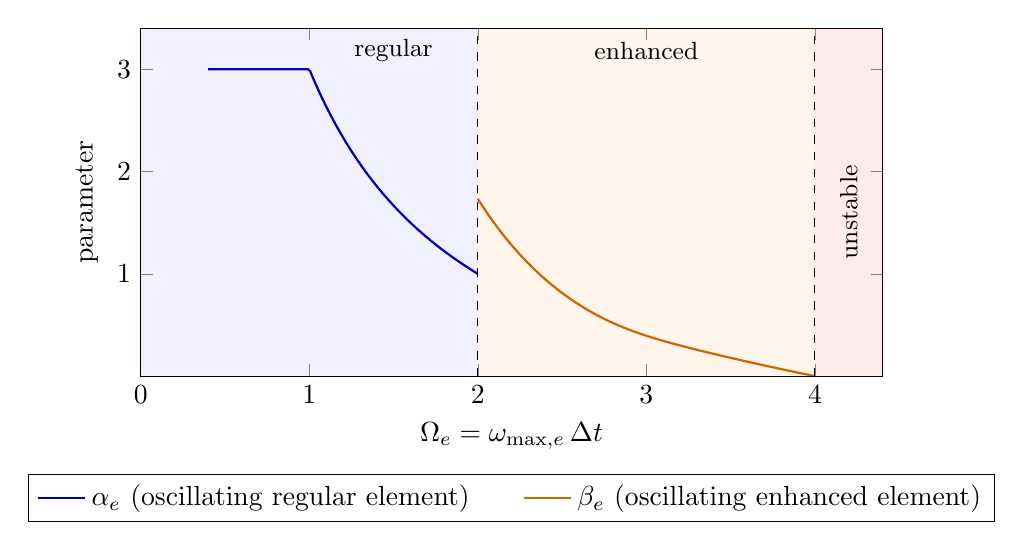
\begin{tikzpicture}
  \begin{axis}[
      width=11cm, height=6cm,
      xmin=0, xmax=4.4, ymin=0, ymax=3.4,
      xlabel={$\Omega_e=\omega_{\max,e}\,\Delta t$},
      ylabel={parameter},
      xtick={0,1,2,3,4}, ytick={1,2,3},
      legend style={at={(0.5,-0.28)}, anchor=north, legend columns=2,
                    /tikz/every even column/.append style={column sep=6mm}},
      legend cell align=left,
      every axis plot/.append style={thick},
      axis on top]
    % regions
    \fill[blue!6] (axis cs:0,0) rectangle (axis cs:2,3.4);
    \fill[orange!8] (axis cs:2,0) rectangle (axis cs:4,3.4);
    \fill[red!8] (axis cs:4,0) rectangle (axis cs:4.4,3.4);
    \node[font=\small] at (axis cs:1.5,3.18) {regular};
    \node[font=\small] at (axis cs:3,3.18) {enhanced};
    \node[font=\small, rotate=90] at (axis cs:4.2,1.6) {unstable};
    % alpha_e = min(3, 4/Omega - 1)
    \addplot[blue!70!black, domain=0.4:2, samples=120]
      {min(3, 4/x - 1)};
    \addlegendentry{$\alpha_e$ (oscillating regular element)}
    % beta_e
    \addplot[orange!80!black, domain=2.0001:4, samples=120]
      {(16 - (x^2-8)^2 + 4*sqrt(16 + 2*(x^2-8)^2))/x^4};
    \addlegendentry{$\beta_e$ (oscillating enhanced element)}
    \draw[dashed] (axis cs:2,0) -- (axis cs:2,3.4);
    \draw[dashed] (axis cs:4,0) -- (axis cs:4,3.4);
  \end{axis}
\end{tikzpicture}

  \caption{Integration parameters of the adaptive hybrid explicit method for
    $\zeta_e = 0$: $\alpha_e$ for oscillating regular elements (Eq.~(8b),
    capped at 3) and $\beta_e$ for oscillating enhanced elements (Eq.~(12b)).}
  \label{fig:ahem}
\end{figure}

\code{tests/integration/AdaptiveHybridExplicitTest.m} checks second-order
convergence, damping, and stable, accurate results at twice the
central-difference limit, where the central difference method diverges.

\section{Excitation signals}
\label{sec:signals}

The function \code{ExcitationSignal} (arguments \code{SignalType},
\code{ExciteParam}, \code{t}) returns the signal as a row vector,
\code{ExcitationSignalDerivative} (additional argument \code{order}) its
derivatives.

\begin{xltabular}{\linewidth}{@{}P{1.9cm}LP{5.0cm}@{}}
  \toprule
  \code{SignalType} & signal & \code{ExciteParam} \\
  \midrule
  0 & none & \code{tE} \\
  1 & sine burst with Hann window $\sin(2\pi f t)\sin^2(\pi f t/n)$ for $t < n/f$
    & \code{[f, n]} \\
  2 & sine with Gaussian window & \code{f} \\
  3 & linear chirp & \code{[f0, f1, t1]} \\
  4 & harmonic $a\cos(2\pi f_0 t) + b\sin(2\pi f_1 t)$ & \code{[a, b, f0, f1]} \\
  5 & piecewise linear & table \code{[t, amplitude; ...; tE, 0]} \\
  6 & Ricker wavelet, delay $1/f$ & \code{f} \\
  7 & Gaussian impulses & \code{[a, b, c, d, n]}: amplitude, first peak, width,
    spacing, number \\
  \bottomrule
\end{xltabular}

\code{DefaultExcitationParameters(SignalType, tE)} returns example parameters
(used if \code{settings.ExciteParam} is empty).
\code{RayleighDamping(omega, zeta, flag_vis)} returns $\alpha$ and $\beta$ such
that $\zeta(\omega) = \alpha/(2\omega) + \beta\omega/2$ matches the targets
(closed form for two frequencies, least squares otherwise).

\section{Modal analysis (\texttt{ModalAnalysis})}

\begin{enumerate}
  \item Assemble $\matr K$ and $\matr M$, apply homogeneous constraints.
  \item Undamped: \code{eigs(K_aa, M_aa, numEigen, EVP_Solver.type)}, giving
    $f = \sqrt{|\lambda|}/(2\pi)$ in Hz. The full \code{eig} is used if
    \code{2*numEigen} exceeds the number of active DOFs. An empty
    \code{EVP_Solver.p} (default) selects \code{max(2*numEigen, 20)}.
  \item Damped: state-space form of
    $\lambda^2\matr M\vect u + \lambda\matr R\vect u + \matr K\vect u = \vect 0$,
    giving $f = |\lambda|/(2\pi)$ in Hz and the displacement part of the
    eigenvectors.
  \item The first mode is plotted (real part).
\end{enumerate}
Because $\matr K$ and $\matr M$ are unsymmetric on distorted meshes, eigenvalues
can be complex.

\section{Frequency-domain analysis (\texttt{FrequencyDomainAnalysis})}

The analysis solves $(\matr K - \omega^2\matr M)\hat{\vect u} = \hat{\vect F}$ for
$\omega = 2\pi f_\mathrm{Harmonic}$. Constant and time-dependent loads are treated
as harmonic loads with unit amplitude. Damping and prescribed displacements are
not taken into account.

\chapter{Test suite}
\label{ch:testing}

The tests use the \texttt{MATLAB} unit test framework (\code{matlab.unittest}) and need
only base \texttt{MATLAB}.
\begin{lstlisting}
cd tests
run_tests                       % unit + integration tests (about 2 minutes)
run_tests('unit')               % only tests/unit
run_tests('integration')        % only tests/integration
run_tests('KnownIssues', true)  % also tests tagged KnownIssue (open bugs)
run_tests('Coverage', true)     % Cobertura coverage report of code/subroutines
\end{lstlisting}
From the command line or in continuous integration:
\begin{lstlisting}[style=shell]
matlab -batch "cd tests; run_tests"
\end{lstlisting}
\code{run_tests} writes \code{tests/results/junit.xml} (and \code{coverage.xml})
and throws an error if a test fails. On GitHub Actions it also reports every
failed test as an annotation on the run page. It temporarily switches off the
automatic creation of a parallel pool, so the \code{parfor} loops run serially;
pass \code{'Parallel', true} to allow a pool. Every test class puts
\code{code/subroutines} (with subfolders, as \code{SetupPaths} does) and
\code{tests/helpers} on the path with a \code{PathFixture}, so single classes can
also be run with \code{runtests}. GitHub Actions runs the suite on every push
(\code{.github/workflows/tests.yml}).

\section{Unit tests (\texorpdfstring{\texttt{tests/unit}}{tests/unit})}

\begin{xltabular}{\linewidth}{@{}P{5.0cm}L@{}}
  \toprule
  class & what is checked \\
  \midrule
  \endhead
  \code{QuadratureTest} & Gauss-Legendre and Gauss-Lobatto rules integrate
    polynomials of degree $2n-1$ exactly; interval mapping; symmetry \\
  \code{NodalDistributionTest} & node distributions: ascending, symmetric,
    endpoints; GLL nodes are roots of $P_p'$; GLC nodes are Chebyshev extrema;
    unknown distributions are rejected \\
  \code{ShapeFunctionsTest} & 1D/2D Lagrange functions: Kronecker property,
    partition of unity, reproduction of polynomials and their derivatives,
    anisotropic degrees; bilinear and Serendipity functions \\
  \code{MetricShapeFunctionsTest} & metric functions: Kronecker property;
    completeness in $(x,y)$ on distorted elements; finite-difference
    derivatives; equality with the parametric functions on parallelograms; frame
    invariance (rotation, translation, scaling) and the frame dependence of
    \code{method = 0}; skew coordinates \\
  \code{MetricHybridTest} & hybrid trial space (\code{method = 2}): Kronecker
    property, completeness in $(x,y)$ with gradients, finite-difference
    derivatives, frame invariance, Newton inversion when no local coordinates are
    given, equality with the parametric functions (and the classical $\matr K_e$) on
    straight-edged elements, unsymmetry on curved ones, Lebesgue constant $<7$ at
    $p=12$; element matrices: rigid-body modes, rank $n_\mathrm{dof}-3$, \code{KMe_2D} =
    \code{Ke_2D}/\code{Me_2D}, diagonal nodal-quadrature mass, total mass;
    \code{ReferenceNodes2D}, \code{Global2LocalNewton} \\
  \code{MetricBasisTest} & bases of the metric Vandermonde matrix: derivatives,
    span, closed-form values, Lagrange basis equals the parametric 1D functions;
    metric functions independent of the basis and frame invariant for every basis;
    $\matr V$ is a permutation matrix on affine elements up to $p=16$, metric =
    parametric and $\matr K_e$ symmetric at high $p$; Kronecker property on a
    curved element at $p=12$ \\
  \code{GeometryMappingTest} & Jacobian (constant for affine maps, finite
    differences, $\det(\matr J)>0$), node interpolation, element area, inverse
    mapping \\
  \code{MaterialTest} & Hooke matrices: symmetry, positive definiteness, Lamé
    constants, plane stress/strain reduction against closed forms, transverse
    isotropy and rotations \\
  \code{ElementMatricesTest} & rigid-body modes in the right and left null space,
    rank $n_\mathrm{dof}-3$, symmetry on parallelograms (identical to the classical element),
    unsymmetry on distorted elements, constant-strain energy, rotation
    invariance $\matr K' = \matr T\matr K\matr T^{\T}$; mass: total mass,
    symmetry, diagonal GLL nodal quadrature, lumping and its fallbacks \\
  \code{TopologyTest} & DOF and edge connectivity, boundary edges, number and
    position of the high-order nodes on distorted 4- and 8-node meshes, corner
    node numbering \\
  \code{TimeIntegrationTest} & 20 integrators on a 2-DOF oscillator: free
    vibration, step load, convergence order, multiple right-hand sides,
    velocity and acceleration of the central difference method \\
  \code{ExcitationAndDampingTest} & excitation signals and their derivatives
    (finite differences), Rayleigh damping parameters \\
  \code{DriverTest} & building blocks of the program flow:
    \code{MaterialMatrices} (isotropic against closed forms, orthotropic Voigt
    order, invalid plane state), \code{AlignPolynomialDegrees} (aligned and
    rotated neighbours), example parameters of every signal; the shared helpers
    of the time integrators (time step rules, load at an instant, initial
    acceleration, expansion to all DOFs, triangular storage) \\
  \code{CodeHygieneTest} & every file in \code{code/} has help text, no two files
    have the same name (one would shadow the other on the path), every entry of
    \code{TimeIntegrationMethods} exists \\
  \bottomrule
\end{xltabular}

\section{Integration tests (\texorpdfstring{\texttt{tests/integration}}{tests/integration})}

The patch tests and the comparison of the trial spaces in
\cref{sec:metric-hybrid} use a $3\times2$ mesh on $[0,3]\times[0,2]$
(\cref{fig:test-meshes}). Only the interior nodes are moved, so the boundary is
the same for all meshes; the displacements of the exact solution are prescribed
at all boundary nodes, and no other loads act.

\begin{figure}[htbp]
  \centering
  % 3 x 2 test meshes (tests/helpers/usemTestMesh.m, usemDistortMesh.m); generated
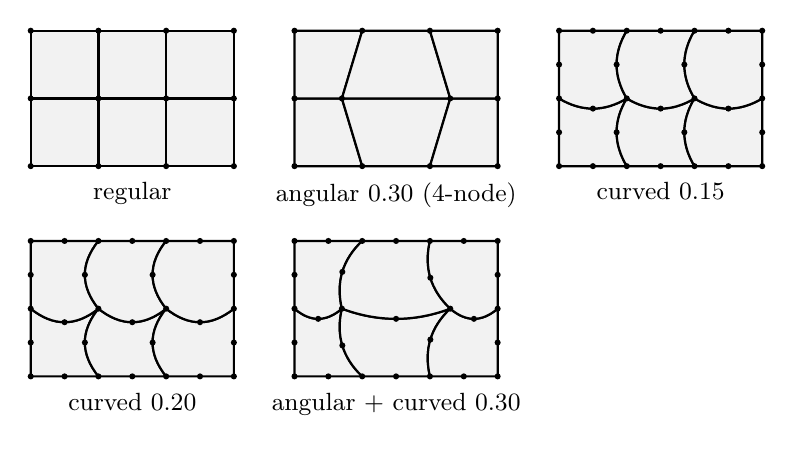
\begin{tikzpicture}[x=0.86cm, y=0.86cm, every node/.style={font=\small}]
  \begin{scope}[xshift=0.00cm, yshift=-0.00cm]
    \draw[thick, fill=black!5] (0.0000,0.0000) -- (1.0000,0.0000) -- (1.0000,1.0000) -- (0.0000,1.0000) -- cycle;
    \draw[thick, fill=black!5] (1.0000,0.0000) -- (2.0000,0.0000) -- (2.0000,1.0000) -- (1.0000,1.0000) -- cycle;
    \draw[thick, fill=black!5] (2.0000,0.0000) -- (3.0000,0.0000) -- (3.0000,1.0000) -- (2.0000,1.0000) -- cycle;
    \draw[thick, fill=black!5] (0.0000,1.0000) -- (1.0000,1.0000) -- (1.0000,2.0000) -- (0.0000,2.0000) -- cycle;
    \draw[thick, fill=black!5] (1.0000,1.0000) -- (2.0000,1.0000) -- (2.0000,2.0000) -- (1.0000,2.0000) -- cycle;
    \draw[thick, fill=black!5] (2.0000,1.0000) -- (3.0000,1.0000) -- (3.0000,2.0000) -- (2.0000,2.0000) -- cycle;
    \fill (0.0000,0.0000) circle (1.1pt);
    \fill (1.0000,0.0000) circle (1.1pt);
    \fill (2.0000,0.0000) circle (1.1pt);
    \fill (3.0000,0.0000) circle (1.1pt);
    \fill (0.0000,1.0000) circle (1.1pt);
    \fill (1.0000,1.0000) circle (1.1pt);
    \fill (2.0000,1.0000) circle (1.1pt);
    \fill (3.0000,1.0000) circle (1.1pt);
    \fill (0.0000,2.0000) circle (1.1pt);
    \fill (1.0000,2.0000) circle (1.1pt);
    \fill (2.0000,2.0000) circle (1.1pt);
    \fill (3.0000,2.0000) circle (1.1pt);
    \node[below] at (1.5,-0.1) {regular};
  \end{scope}
  \begin{scope}[xshift=3.35cm, yshift=-0.00cm]
    \draw[thick, fill=black!5] (0.0000,0.0000) -- (1.0000,0.0000) -- (0.7000,1.0000) -- (0.0000,1.0000) -- cycle;
    \draw[thick, fill=black!5] (1.0000,0.0000) -- (2.0000,0.0000) -- (2.3000,1.0000) -- (0.7000,1.0000) -- cycle;
    \draw[thick, fill=black!5] (2.0000,0.0000) -- (3.0000,0.0000) -- (3.0000,1.0000) -- (2.3000,1.0000) -- cycle;
    \draw[thick, fill=black!5] (0.0000,1.0000) -- (0.7000,1.0000) -- (1.0000,2.0000) -- (0.0000,2.0000) -- cycle;
    \draw[thick, fill=black!5] (0.7000,1.0000) -- (2.3000,1.0000) -- (2.0000,2.0000) -- (1.0000,2.0000) -- cycle;
    \draw[thick, fill=black!5] (2.3000,1.0000) -- (3.0000,1.0000) -- (3.0000,2.0000) -- (2.0000,2.0000) -- cycle;
    \fill (0.0000,0.0000) circle (1.1pt);
    \fill (1.0000,0.0000) circle (1.1pt);
    \fill (2.0000,0.0000) circle (1.1pt);
    \fill (3.0000,0.0000) circle (1.1pt);
    \fill (0.0000,1.0000) circle (1.1pt);
    \fill (0.7000,1.0000) circle (1.1pt);
    \fill (2.3000,1.0000) circle (1.1pt);
    \fill (3.0000,1.0000) circle (1.1pt);
    \fill (0.0000,2.0000) circle (1.1pt);
    \fill (1.0000,2.0000) circle (1.1pt);
    \fill (2.0000,2.0000) circle (1.1pt);
    \fill (3.0000,2.0000) circle (1.1pt);
    \node[below] at (1.5,-0.1) {angular 0.30 (4-node)};
  \end{scope}
  \begin{scope}[xshift=6.71cm, yshift=-0.00cm]
    \draw[thick, fill=black!5] (0.0000,0.0000) .. controls (0.3333,0.0000) and (0.6667,0.0000) .. (1.0000,0.0000) .. controls (0.8000,0.3333) and (0.8000,0.6667) .. (1.0000,1.0000) .. controls (0.6667,0.8000) and (0.3333,0.8000) .. (0.0000,1.0000) .. controls (0.0000,0.6667) and (0.0000,0.3333) .. (0.0000,0.0000) -- cycle;
    \draw[thick, fill=black!5] (1.0000,0.0000) .. controls (1.3333,0.0000) and (1.6667,0.0000) .. (2.0000,0.0000) .. controls (1.8000,0.3333) and (1.8000,0.6667) .. (2.0000,1.0000) .. controls (1.6667,0.8000) and (1.3333,0.8000) .. (1.0000,1.0000) .. controls (0.8000,0.6667) and (0.8000,0.3333) .. (1.0000,0.0000) -- cycle;
    \draw[thick, fill=black!5] (2.0000,0.0000) .. controls (2.3333,0.0000) and (2.6667,0.0000) .. (3.0000,0.0000) .. controls (3.0000,0.3333) and (3.0000,0.6667) .. (3.0000,1.0000) .. controls (2.6667,0.8000) and (2.3333,0.8000) .. (2.0000,1.0000) .. controls (1.8000,0.6667) and (1.8000,0.3333) .. (2.0000,0.0000) -- cycle;
    \draw[thick, fill=black!5] (0.0000,1.0000) .. controls (0.3333,0.8000) and (0.6667,0.8000) .. (1.0000,1.0000) .. controls (0.8000,1.3333) and (0.8000,1.6667) .. (1.0000,2.0000) .. controls (0.6667,2.0000) and (0.3333,2.0000) .. (0.0000,2.0000) .. controls (0.0000,1.6667) and (0.0000,1.3333) .. (0.0000,1.0000) -- cycle;
    \draw[thick, fill=black!5] (1.0000,1.0000) .. controls (1.3333,0.8000) and (1.6667,0.8000) .. (2.0000,1.0000) .. controls (1.8000,1.3333) and (1.8000,1.6667) .. (2.0000,2.0000) .. controls (1.6667,2.0000) and (1.3333,2.0000) .. (1.0000,2.0000) .. controls (0.8000,1.6667) and (0.8000,1.3333) .. (1.0000,1.0000) -- cycle;
    \draw[thick, fill=black!5] (2.0000,1.0000) .. controls (2.3333,0.8000) and (2.6667,0.8000) .. (3.0000,1.0000) .. controls (3.0000,1.3333) and (3.0000,1.6667) .. (3.0000,2.0000) .. controls (2.6667,2.0000) and (2.3333,2.0000) .. (2.0000,2.0000) .. controls (1.8000,1.6667) and (1.8000,1.3333) .. (2.0000,1.0000) -- cycle;
    \fill (0.0000,0.0000) circle (1.1pt);
    \fill (1.0000,0.0000) circle (1.1pt);
    \fill (2.0000,0.0000) circle (1.1pt);
    \fill (3.0000,0.0000) circle (1.1pt);
    \fill (0.0000,1.0000) circle (1.1pt);
    \fill (1.0000,1.0000) circle (1.1pt);
    \fill (2.0000,1.0000) circle (1.1pt);
    \fill (3.0000,1.0000) circle (1.1pt);
    \fill (0.0000,2.0000) circle (1.1pt);
    \fill (1.0000,2.0000) circle (1.1pt);
    \fill (2.0000,2.0000) circle (1.1pt);
    \fill (3.0000,2.0000) circle (1.1pt);
    \fill (0.5000,0.0000) circle (1.1pt);
    \fill (0.8500,0.5000) circle (1.1pt);
    \fill (0.5000,0.8500) circle (1.1pt);
    \fill (0.0000,0.5000) circle (1.1pt);
    \fill (1.5000,0.0000) circle (1.1pt);
    \fill (1.8500,0.5000) circle (1.1pt);
    \fill (1.5000,0.8500) circle (1.1pt);
    \fill (2.5000,0.0000) circle (1.1pt);
    \fill (3.0000,0.5000) circle (1.1pt);
    \fill (2.5000,0.8500) circle (1.1pt);
    \fill (0.8500,1.5000) circle (1.1pt);
    \fill (0.5000,2.0000) circle (1.1pt);
    \fill (0.0000,1.5000) circle (1.1pt);
    \fill (1.8500,1.5000) circle (1.1pt);
    \fill (1.5000,2.0000) circle (1.1pt);
    \fill (3.0000,1.5000) circle (1.1pt);
    \fill (2.5000,2.0000) circle (1.1pt);
    \node[below] at (1.5,-0.1) {curved 0.15};
  \end{scope}
  \begin{scope}[xshift=0.00cm, yshift=-2.67cm]
    \draw[thick, fill=black!5] (0.0000,0.0000) .. controls (0.3333,0.0000) and (0.6667,0.0000) .. (1.0000,0.0000) .. controls (0.7333,0.3333) and (0.7333,0.6667) .. (1.0000,1.0000) .. controls (0.6667,0.7333) and (0.3333,0.7333) .. (0.0000,1.0000) .. controls (0.0000,0.6667) and (0.0000,0.3333) .. (0.0000,0.0000) -- cycle;
    \draw[thick, fill=black!5] (1.0000,0.0000) .. controls (1.3333,0.0000) and (1.6667,0.0000) .. (2.0000,0.0000) .. controls (1.7333,0.3333) and (1.7333,0.6667) .. (2.0000,1.0000) .. controls (1.6667,0.7333) and (1.3333,0.7333) .. (1.0000,1.0000) .. controls (0.7333,0.6667) and (0.7333,0.3333) .. (1.0000,0.0000) -- cycle;
    \draw[thick, fill=black!5] (2.0000,0.0000) .. controls (2.3333,0.0000) and (2.6667,0.0000) .. (3.0000,0.0000) .. controls (3.0000,0.3333) and (3.0000,0.6667) .. (3.0000,1.0000) .. controls (2.6667,0.7333) and (2.3333,0.7333) .. (2.0000,1.0000) .. controls (1.7333,0.6667) and (1.7333,0.3333) .. (2.0000,0.0000) -- cycle;
    \draw[thick, fill=black!5] (0.0000,1.0000) .. controls (0.3333,0.7333) and (0.6667,0.7333) .. (1.0000,1.0000) .. controls (0.7333,1.3333) and (0.7333,1.6667) .. (1.0000,2.0000) .. controls (0.6667,2.0000) and (0.3333,2.0000) .. (0.0000,2.0000) .. controls (0.0000,1.6667) and (0.0000,1.3333) .. (0.0000,1.0000) -- cycle;
    \draw[thick, fill=black!5] (1.0000,1.0000) .. controls (1.3333,0.7333) and (1.6667,0.7333) .. (2.0000,1.0000) .. controls (1.7333,1.3333) and (1.7333,1.6667) .. (2.0000,2.0000) .. controls (1.6667,2.0000) and (1.3333,2.0000) .. (1.0000,2.0000) .. controls (0.7333,1.6667) and (0.7333,1.3333) .. (1.0000,1.0000) -- cycle;
    \draw[thick, fill=black!5] (2.0000,1.0000) .. controls (2.3333,0.7333) and (2.6667,0.7333) .. (3.0000,1.0000) .. controls (3.0000,1.3333) and (3.0000,1.6667) .. (3.0000,2.0000) .. controls (2.6667,2.0000) and (2.3333,2.0000) .. (2.0000,2.0000) .. controls (1.7333,1.6667) and (1.7333,1.3333) .. (2.0000,1.0000) -- cycle;
    \fill (0.0000,0.0000) circle (1.1pt);
    \fill (1.0000,0.0000) circle (1.1pt);
    \fill (2.0000,0.0000) circle (1.1pt);
    \fill (3.0000,0.0000) circle (1.1pt);
    \fill (0.0000,1.0000) circle (1.1pt);
    \fill (1.0000,1.0000) circle (1.1pt);
    \fill (2.0000,1.0000) circle (1.1pt);
    \fill (3.0000,1.0000) circle (1.1pt);
    \fill (0.0000,2.0000) circle (1.1pt);
    \fill (1.0000,2.0000) circle (1.1pt);
    \fill (2.0000,2.0000) circle (1.1pt);
    \fill (3.0000,2.0000) circle (1.1pt);
    \fill (0.5000,0.0000) circle (1.1pt);
    \fill (0.8000,0.5000) circle (1.1pt);
    \fill (0.5000,0.8000) circle (1.1pt);
    \fill (0.0000,0.5000) circle (1.1pt);
    \fill (1.5000,0.0000) circle (1.1pt);
    \fill (1.8000,0.5000) circle (1.1pt);
    \fill (1.5000,0.8000) circle (1.1pt);
    \fill (2.5000,0.0000) circle (1.1pt);
    \fill (3.0000,0.5000) circle (1.1pt);
    \fill (2.5000,0.8000) circle (1.1pt);
    \fill (0.8000,1.5000) circle (1.1pt);
    \fill (0.5000,2.0000) circle (1.1pt);
    \fill (0.0000,1.5000) circle (1.1pt);
    \fill (1.8000,1.5000) circle (1.1pt);
    \fill (1.5000,2.0000) circle (1.1pt);
    \fill (3.0000,1.5000) circle (1.1pt);
    \fill (2.5000,2.0000) circle (1.1pt);
    \node[below] at (1.5,-0.1) {curved 0.20};
  \end{scope}
  \begin{scope}[xshift=3.35cm, yshift=-2.67cm]
    \draw[thick, fill=black!5] (0.0000,0.0000) .. controls (0.3333,0.0000) and (0.6667,0.0000) .. (1.0000,0.0000) .. controls (0.7084,0.2759) and (0.6084,0.6092) .. (0.7000,1.0000) .. controls (0.4667,0.8000) and (0.2333,0.8000) .. (0.0000,1.0000) .. controls (0.0000,0.6667) and (0.0000,0.3333) .. (0.0000,0.0000) -- cycle;
    \draw[thick, fill=black!5] (1.0000,0.0000) .. controls (1.3333,0.0000) and (1.6667,0.0000) .. (2.0000,0.0000) .. controls (1.9084,0.3908) and (2.0084,0.7241) .. (2.3000,1.0000) .. controls (1.7667,0.8000) and (1.2333,0.8000) .. (0.7000,1.0000) .. controls (0.6084,0.6092) and (0.7084,0.2759) .. (1.0000,0.0000) -- cycle;
    \draw[thick, fill=black!5] (2.0000,0.0000) .. controls (2.3333,0.0000) and (2.6667,0.0000) .. (3.0000,0.0000) .. controls (3.0000,0.3333) and (3.0000,0.6667) .. (3.0000,1.0000) .. controls (2.7667,0.8000) and (2.5333,0.8000) .. (2.3000,1.0000) .. controls (2.0084,0.7241) and (1.9084,0.3908) .. (2.0000,0.0000) -- cycle;
    \draw[thick, fill=black!5] (0.0000,1.0000) .. controls (0.2333,0.8000) and (0.4667,0.8000) .. (0.7000,1.0000) .. controls (0.6084,1.3908) and (0.7084,1.7241) .. (1.0000,2.0000) .. controls (0.6667,2.0000) and (0.3333,2.0000) .. (0.0000,2.0000) .. controls (0.0000,1.6667) and (0.0000,1.3333) .. (0.0000,1.0000) -- cycle;
    \draw[thick, fill=black!5] (0.7000,1.0000) .. controls (1.2333,0.8000) and (1.7667,0.8000) .. (2.3000,1.0000) .. controls (2.0084,1.2759) and (1.9084,1.6092) .. (2.0000,2.0000) .. controls (1.6667,2.0000) and (1.3333,2.0000) .. (1.0000,2.0000) .. controls (0.7084,1.7241) and (0.6084,1.3908) .. (0.7000,1.0000) -- cycle;
    \draw[thick, fill=black!5] (2.3000,1.0000) .. controls (2.5333,0.8000) and (2.7667,0.8000) .. (3.0000,1.0000) .. controls (3.0000,1.3333) and (3.0000,1.6667) .. (3.0000,2.0000) .. controls (2.6667,2.0000) and (2.3333,2.0000) .. (2.0000,2.0000) .. controls (1.9084,1.6092) and (2.0084,1.2759) .. (2.3000,1.0000) -- cycle;
    \fill (0.0000,0.0000) circle (1.1pt);
    \fill (1.0000,0.0000) circle (1.1pt);
    \fill (2.0000,0.0000) circle (1.1pt);
    \fill (3.0000,0.0000) circle (1.1pt);
    \fill (0.0000,1.0000) circle (1.1pt);
    \fill (0.7000,1.0000) circle (1.1pt);
    \fill (2.3000,1.0000) circle (1.1pt);
    \fill (3.0000,1.0000) circle (1.1pt);
    \fill (0.0000,2.0000) circle (1.1pt);
    \fill (1.0000,2.0000) circle (1.1pt);
    \fill (2.0000,2.0000) circle (1.1pt);
    \fill (3.0000,2.0000) circle (1.1pt);
    \fill (0.5000,0.0000) circle (1.1pt);
    \fill (0.7063,0.4569) circle (1.1pt);
    \fill (0.3500,0.8500) circle (1.1pt);
    \fill (0.0000,0.5000) circle (1.1pt);
    \fill (1.5000,0.0000) circle (1.1pt);
    \fill (2.0063,0.5431) circle (1.1pt);
    \fill (1.5000,0.8500) circle (1.1pt);
    \fill (2.5000,0.0000) circle (1.1pt);
    \fill (3.0000,0.5000) circle (1.1pt);
    \fill (2.6500,0.8500) circle (1.1pt);
    \fill (0.7063,1.5431) circle (1.1pt);
    \fill (0.5000,2.0000) circle (1.1pt);
    \fill (0.0000,1.5000) circle (1.1pt);
    \fill (2.0063,1.4569) circle (1.1pt);
    \fill (1.5000,2.0000) circle (1.1pt);
    \fill (3.0000,1.5000) circle (1.1pt);
    \fill (2.5000,2.0000) circle (1.1pt);
    \node[below] at (1.5,-0.1) {angular + curved 0.30};
  \end{scope}
\end{tikzpicture}

  \caption{$3\times2$ test meshes (\texttt{usemTestMesh}, \texttt{usemDistortMesh}):
    4-node meshes (regular, angular distortion 0.30) and 8-node meshes with
    curved-edge distortion (mid-side nodes moved normal to their edge by 0.15 or
    0.20) and with combined angular and curved-edge distortion. Dots: nodes of
    the input mesh. Boundary condition: prescribed displacements on the whole
    boundary.}
  \label{fig:test-meshes}
\end{figure}

\begin{xltabular}{\linewidth}{@{}P{5.0cm}L@{}}
  \toprule
  class & what is checked \\
  \midrule
  \endhead
  \code{PatchTest} & displacement patch tests on regular, angular, curved and
    combined distorted meshes for $p = 1,\dots,4$, plane stress and plane strain:
    linear fields, all harmonic fields $(\operatorname{Re}(z^k), -\operatorname{Im}
    (z^k))$ with $k\le p$, and pure bending are reproduced to machine precision.
    Control experiment: the classical symmetric element fails on the same curved
    mesh. Fields of higher degree are not exact; exponential $p$-convergence for
    $(e^x\cos(y), -e^x\sin(y))$. All exactness and convergence tests run for both
    trial spaces (\code{method} 1 and 2); the hybrid element equals the classical one
    on the angular mesh and is unsymmetric on the curved mesh \\
  \code{RunSimulationTest} & the complete program flow from the input file:
    static result against the stored reference solution, modal analysis against
    the dense eigenvalues of the returned matrices, frequency-domain solution for
    $\omega\to0$ against the static one, transient analysis (Newmark), saved
    files (results, $u_y$ export, solver input that reproduces the time
    integration), errors for an unknown analysis type and a missing input file \\
  \code{LeeBathePatchTest} & the Lee-Bathe patch tests (reference data in
    \code{tests/fixtures/reference}), repeated with the steps of
    \code{StaticAnalysis}: the quadratic test matches the analytical pure-bending
    solution for all meshes and $p\ge2$; the cubic test for $p = 3$ is
    mesh-independent and matches the stored solution; both trial spaces \\
  \code{AbaqusInputTest} & end to end: the input files in
    \code{code/InputFilesAbaqus} are read with \code{ReadModel}, lifted to degree
    $p$ and compared with the reference models; static analysis from the input
    file \\
  \code{AbaqusReaderTest} & reader robustness with modified input files: exact set
    names (\code{Set-1} vs.\ \code{Set-10}), missing sets (error instead of an
    endless loop), U2 + U3 in separate lines, \texttt{\%} in the file, node labels,
    gravity, \code{*Cload} on a generated set \\
  \code{DirichletBCTest} & homogeneous and prescribed displacements
    (elimination), uniaxial stretch on a distorted mesh, node sets used as given \\
  \code{LoadsTest} & body forces on element subsets, several body forces, gravity
    with the density of each material, one or several load cases, amplitude of
    spatially varying loads \\
  \code{SolverTransientTest} & \code{Solver_Transient} with the input struct of
    \code{DynamicAnalysis} or its MAT file: methods 301, 306, 202, 402, 403
    (undamped and damped Padé, also from rest under a constant load), 109 with
    element data (and the error without), all DOFs saved with
    \code{save_var = 1}, Newmark fallback (with a warning) for unknown codes,
    unique method codes \\
  \code{AdaptiveHybridExplicitTest} & adaptive hybrid explicit method:
    second-order convergence, mass-proportional damping against the exact
    solution, stable and accurate at twice the critical time step of the central
    difference method (which diverges), diagonal lumped mass \\
  \bottomrule
\end{xltabular}

\section{Helpers and fixtures}

\begin{xltabular}{\linewidth}{@{}P{5.0cm}L@{}}
  \toprule
  file & purpose \\
  \midrule
  \code{helpers/usemTestMesh} & structured 4- or 8-node mesh in \texttt{ABAQUS} node order \\
  \code{helpers/usemDistortMesh} & deterministic angular, curved-edge or combined
    distortion of interior nodes \\
  \code{helpers/usemTestElement} & single test elements (square, parallelogram,
    trapezoid, curved, general) \\
  \code{helpers/usemBuildModel} & wrapper of \code{pSpectralElement_NodesTopology} \\
  \code{helpers/usemAssemble} & quiet wrapper of \code{AssemblyFEM} \\
  \code{helpers/usemDirichletSolve} & displacement-driven patch test \\
  \code{helpers/usemKeSymmetric} & classical (Bubnov-Galerkin) element stiffness,
    for comparisons only \\
  \code{helpers/usemReadAbaqus} & \code{ReadModel} without progress output (used
    by the studies) \\
  \code{fixtures/reference/*.mat} & model data and solutions of the Lee-Bathe
    tests, extracted from the result workspaces in
    \code{code/subroutines/Results/Static} (\code{make_reference_fixtures.m}) \\
  \code{fixtures/make_abaqus_inputs.m} & generation of the \texttt{ABAQUS} input files
    from the fixtures \\
  \bottomrule
\end{xltabular}

\section{Writing new tests}

\begin{itemize}
  \item Put the new class in \code{tests/unit} or \code{tests/integration} and copy
    the \code{TestClassSetup} block (path fixtures) from an existing class.
  \item Wrap routines that print progress (\code{AssemblyFEM}, \code{NeumannBCs},
    integrators, \code{RunSimulation}) in \code{evalc}, or use the helpers that
    already do this; for \code{RunSimulation} also set \code{settings.verbose},
    \code{settings.parallel}, \code{settings.saveWS} and the plot flags to
    \code{false}.
  \item Numerical changes that should not change results (refactoring) can be
    checked bit for bit against the unmodified code: run both versions on the
    same input and compare with \code{isequal}, as \code{RunSimulationTest} and
    \code{SolverTransientTest} do for files written by the program.
  \item Use deterministic meshes (\code{usemDistortMesh}) or a seeded
    \code{RandStream}.
  \item Use only base \texttt{MATLAB} functions (the GitHub runner has no toolboxes).
  \item Tag tests that document an unfixed bug with
    \code{TestTags = {'KnownIssue'}} and describe the bug in \cref{ch:issues}.
\end{itemize}

\chapter{Known limitations}
\label{ch:issues}

\begin{itemize}
  \item \textbf{Mesh reader.} \code{Read_mesh_ABAQUS} reads the \code{*Node} block and
    the first \code{*Element} block of the 8-node meshes of the two studies; node
    labels are used as row numbers, and the corner nodes must be numbered first
    (\code{pSpectralElement_NodesTopology} checks this).
  \item \textbf{Geometry.} The element geometry is that of the 4-node or 8-node
    input mesh, whatever the polynomial degree: the elements are subparametric for
    $p>2$, and curved boundaries do not become more accurate under
    $p$-refinement. Only the thick-cylinder study places the nodes of the arcs on the
    exact geometry (\cref{ch:theory}).
  \item \textbf{Numerical integration.} $2p$ Gauss points per direction do not
    integrate the element matrices of curved elements exactly
    (\cref{sec:quadrature}); the patch tests are not affected. The mesh-level studies
    use calibrated rules.
\end{itemize}

\chapter{Literature}
\label{ch:literature}

This chapter collects the literature on the unsymmetric finite element method
(UFEM) that the code is built on. All entries are in
\code{literature/references.bib}; the full references with DOIs are listed at the
end of this document. The PDFs are not under version control because they are
publisher-copyrighted or unpublished.

Element acronyms: PP = parametric test / parametric trial (classical
isoparametric); PM = parametric test / metric trial (unsymmetric, ``US-''); MM =
metric / metric; ATF = analytical trial functions.

\section{References followed by the implementation}

\begin{xltabular}{\linewidth}{@{}LP{6.2cm}@{}}
  \toprule
  code & references \\
  \midrule
  unsymmetric (Petrov--Galerkin) element, adjugate form of $\matr B_L$
    (\code{Ke_2D}, \code{Me_2D}, \code{KMe_2D}) &
    \textcite{Rajendran2010technique}; \textcite{Rajendran2003novel} \\
  metric trial functions in corotational skew coordinates
    (\code{ShapeFunctions2D_Metric}, \code{CorotationalSkewCoordinates}) &
    \textcite{Xie2016Modified}; \textcite{Yuan1993New};
    \textcite{Ooi2008Remedies} \\
  Lee \& Bathe patch tests (\code{code/InputFilesAbaqus},
    \code{SpatialLoadingFunction}) &
    \textcite{Lee1993effects}; \textcite{Rajendran2003novel} \\
  adaptive hybrid explicit method (\code{AdaptiveHybridExplicitMethod}) &
    \textcite{Soares2020novel} \\
  stability of time integration with unsymmetric matrices &
    \textcite{Wang2022Temporal}; \textcite{Zaehringer2026On} \\
  \bottomrule
\end{xltabular}

\section{Annotated bibliography}

% Two-column table: reference and key content
\newcommand{\littable}[1]{%
  \begin{xltabular}{\linewidth}{@{}P{4.4cm}L@{}}
    \toprule
    reference & key content \\
    \midrule
    \endhead
    #1
    \bottomrule
  \end{xltabular}}

\subsection{Axisymmetric UFEM}
\littable{
  \textcite{Zaehringer2024finite} & 8-node PG-Q8: serendipity test functions, metric
    trial functions in skew coordinates. Exact for quadratic fields on distorted
    meshes; for the thick-walled cylinder (non-polynomial $u_r$) not generally
    better than Q8. \\
  \textcite{Dou2025novel} & UQ4-RPIM; extension to axisymmetry with a modified
    polynomial basis for hollow bodies. \\
  \textcite{Huang2020incompatible} & IUQ4; axisymmetric extension with incompatible
    test modes that pass the axisymmetric patch test. \\
}

\subsection{Foundations of UFEM and Petrov--Galerkin elements}
\littable{
  \textcite{Rajendran2003novel} & US-QUAD8, the seminal paper: serendipity
    (compatibility-enforcing) test functions with metric (completeness-enforcing)
    trial functions; exact quadratic fields under angular, curved-edge and
    mid-node distortion. \\
  \textcite{Rajendran2000completeness} & higher-order completeness conditions;
    why distorted Q8 elements lose quadratic completeness. \\
  \textcite{Rajendran2010technique} & three sufficient conditions for distortion
    immunity (compatible test, complete trial, no $\det\matr J$ in the
    denominator); PP/PM/MM naming. \\
  \textcite{Ooi2006unsymmetric} & comprehensive study of US-QUAD8/US-HEXA20:
    strong-form patch tests, geometric nonlinearity, frame dependence, P-matrix
    singularity, complex eigenvalues. \\
  \textcite{Prathap2007The} & the PM formulation is not variationally correct but
    recovers stresses as a best fit in metric space. \\
  \textcite{Cen2019Some} & review of hybrid stress/displacement-function elements
    and the improved UFEM (US-ATF family). \\
  \textcite{Chen2021implementierung} & Abaqus UEL implementation of PM-QUAD8 and
    PM-HEXA20; cantilever and Kirsch-plate benchmarks under distortion. \\
}

\subsection{Skew coordinates and frame invariance}
\littable{
  \textcite{Xie2016Modified} & UQ8*, a frame-invariant UQ8 with metric trial
    functions in non-dimensional skew coordinates; Trefftz-UFEM TQ4/TH8. \\
  \textcite{Yuan1993New} & origin of the skew (oblique) coordinates defined at the
    element centre. \\
  \textcite{Ooi2008Remedies} & US-QUAD8 is frame-dependent for the cubic terms and
    its P-matrix can become singular; remedies. \\
  \textcite{Cowan2014Rotationally} & metric trial functions in a local convected
    frame (rotational invariance); finite-deformation elasto-plasticity. \\
  \textcite{Wisniewski2008improved} & Hellinger--Reissner 4-node elements with
    stresses in skew coordinates. \\
}

\subsection{Plane elements}
\littable{
  \textcite{Rajendran2004mesh} & comparison of PP, MM, PM and MP 8-node elements. \\
  \textcite{Liew2006quadratic} & US-TRIA6; free vibration with an unsymmetric mass
    matrix. \\
  \textcite{Cen2012shape} & US-ATFQ8 with Airy-function analytical trial functions. \\
  \textcite{Cen2015unsymmetric} & US-ATFQ4, ``breaking through'' MacNeal's
    theorem. \\
  \textcite{Shang2018quadrilateral} & US-Q4 with drilling DOFs and stress trial
    functions. \\
  \textcite{Shang2018airy} & US-Q8 for orthotropic problems (Airy stress
    solutions). \\
  \textcite{Huang2022Unsymmetric} & UQ6, UH11: Wilson incompatible modes, explicit
    trial functions. \\
  \textcite{Yang2023Two} & UQ10, UQ10/E4: cubic completeness through incompatible
    modes / EAS. \\
}

\subsection{Solid and solid-shell elements}
\littable{
  \textcite{Ooi2004hexahedron} & US-HEXA20. \\
  \textcite{Zhou2017unsymmetric} & US-ATFH8. \\
  \textcite{Huang2018unsymmetric} & US-ATFHS8 solid-shell. \\
  \textcite{Wu2023unsymmetric} & UHS11 solid-shell. \\
  \textcite{He2019generalized} & generalized modal element method (US-MEM8S). \\
  \textcite{Pfefferkorn2021mesh} & Petrov--Galerkin EAS (Q1U/E4, H1U/E12);
    MacNeal's theorem revisited. \\
}

\subsection{Nonlinear extensions}
\littable{
  \textcite{Ooi2007extension} & US-QUAD8/US-HEXA20, total Lagrangian. \\
  \textcite{Li2018high} & US-ATFQ4, updated Lagrangian. \\
  \textcite{Li2019unsymmetric} & US-ATFHS8, corotational. \\
  \textcite{Li2020hyperelastic} & US-ATFQ4, hyperelastic. \\
  \textcite{Chen2021unsymmetric} & US-QUAD8, elasto-plastic. \\
  \textcite{Pfefferkorn2023hourglassing} & PG-EAS H1U/h12, large deformations. \\
  \textcite{Wang2023high} & US-ATFH8 for soft tissues. \\
  \textcite{Wu2026unsymmetric} & UHS11, hyperelastic. \\
}

\subsection{Dynamics and time integration}
\littable{
  \textcite{Wang2022Temporal} & with non-symmetric $\matr M$/$\matr K$ energy is not
    conserved and Newmark can be unconditionally unstable; energy-conserving
    scheme. \\
  \textcite{Zaehringer2026On} & UQ8* in elastodynamics: standard Newmark is
    unstable, Wang--Hillman can drift, a mixed velocity--strain formulation
    conserves energy and stays distortion-insensitive. \\
  \textcite{Kumar2011Use} & transient (impact) application of PM20 with Newmark. \\
  \textcite{Soares2020novel} & adaptive hybrid explicit method (method 109). \\
}

\subsection{Plates, beams and shells}
\littable{
  \textcite{Ju2025unsymmetric} & UQP4-RPIM Reissner--Mindlin plate. \\
  \textcite{Shang2022Trefftz} & US-TP4 Trefftz plate element. \\
}

\subsection{Couple-stress and flexoelectric continua}
\littable{
  \textcite{Shang2019simple} & US-Q4-CS. \\
  \textcite{Shang2020hexahedral} & 8-node hexahedron (modified couple stress). \\
  \textcite{Shang2022couple} & US-Q8, US-Q8L. \\
  \textcite{Wu2023Penalty} & penalty $C^0$ Q8/H20 (consistent couple stress). \\
  \textcite{Deng2025corotational} & corotational flexoelectric membrane. \\
  \textcite{Shang2025Mesh} & Trefftz Kirchhoff plate (consistent couple stress). \\
}

\subsection{Mesh distortion: theory and assessment}
\littable{
  \textcite{Lee1993effects} & angular distortion destroys the quadratic
    completeness of serendipity elements. \\
  \textcite{MacNeal1992On} & MacNeal's theorem: a symmetric element must either
    fail the patch test or lock. \\
  \textcite{Rajendran2007Mesh} & strong-form patch tests; only PM-QUAD8 passes all. \\
  \textcite{Prathap2006mesh} & best-fit paradigm explanation of the distortion
    immunity of PM elements. \\
  \textcite{Mukherjee2011improved} & variationally correct, distortion-immune
    3-node bar. \\
  \textcite{Manju2019function} & function-space analysis of the distorted 3-node
    Timoshenko metric beam. \\
  \textcite{Engvall2020Mesh} & mesh quality metrics for high-order
    (Bernstein--Bézier) elements. \\
  \textcite{Quiriny2024The} & tempered FEM: a lower bound on $\det\matr J$ instead of
    a change of test/trial spaces. \\
  \textcite{Quiriny2026Taming} & tempered FEM for sliver tetrahedra. \\
}

\section{Synthesis}

\begin{enumerate}
  \item \textbf{Why UFEM.} Conventional (Bubnov--Galerkin) serendipity elements lose
    their quadratic completeness under angular and curved-edge distortion
    \parencite{Lee1993effects}. MacNeal's theorem shows that no symmetric element
    can both pass the patch test and be distortion-insensitive in bending
    \parencite{MacNeal1992On}. Petrov--Galerkin elements avoid this by combining
    compatible (parametric) test functions with Cartesian-complete (metric) trial
    functions \parencite{Rajendran2003novel,Rajendran2010technique}.
  \item \textbf{Sufficient conditions for distortion immunity}
    \parencite{Rajendran2010technique}: compatible test functions, trial functions
    complete in Cartesian coordinates, no $\det\matr J$ in the denominator of the
    integrand. This code meets all three for arbitrary $p$: the trial functions are
    tensor-product Lagrange polynomials in skew coordinates, which contain all
    polynomials of total degree $\le p$ in $(x, y)$, and $\matr B_L$ is built with
    $\adj\matr J$. Any displacement field of total degree $\le p$ is reproduced
    exactly on arbitrarily distorted meshes (\code{tests/integration/PatchTest.m}).
  \item \textbf{Frame invariance.} Metric trial functions in global coordinates are
    frame-dependent and their Vandermonde matrix can become singular
    \parencite{Ooi2008Remedies}. Skew coordinates
    \parencite{Yuan1993New,Xie2016Modified} fix the frame dependence; they are the
    default here. The Vandermonde matrix can still be ill-conditioned for
    degenerate elements, e.g.\ three nearly collinear corners.
  \item \textbf{Variational inconsistency.} The PM formulation is not variationally
    correct \parencite{Prathap2007The}: the stiffness matrix is unsymmetric and the
    energy optimality of Bubnov--Galerkin is lost. For fields outside the trial
    space the unsymmetric element can be slightly less accurate than the classical
    one on coarse meshes \parencite{Zaehringer2024finite}, but it keeps the optimal
    convergence rate on distorted meshes.
  \item \textbf{Dynamics.} Unsymmetric $\matr K$ (and $\matr M$) break the
    equivalence of energy and momentum conservation; standard Newmark can become
    unstable and generalized eigenvalues can be complex
    \parencite{Wang2022Temporal,Ooi2006unsymmetric,Zaehringer2026On}. With GLL nodes
    and nodal quadrature the unsymmetric mass matrix is nevertheless diagonal,
    because both the parametric and the metric functions are interpolatory at the
    quadrature points.
  \item \textbf{Open questions.} Element-level stability (conditioning of the metric
    Vandermonde matrix, discrete inf-sup constant) on strongly distorted high-order
    elements; energy-consistent time integration for unsymmetric spectral elements;
    a convergence theory for these variationally inconsistent schemes; extension to
    triangles (\code{ShapeFunctions2D_Metric_Tria} is an unfinished start), 3D and
    axisymmetry.
\end{enumerate}


\printbibliography[heading=bibintoc,title={References}]

\end{document}
